\documentclass{article}

\usepackage[numbers,sort &compress]{natbib}
\usepackage[english]{babel}
\usepackage[utf8]{inputenc}
\usepackage{amsmath,amssymb}
\usepackage{parskip}
\usepackage{graphicx}
\usepackage[utf8]{inputenc}
\usepackage[english]{babel}
 
\usepackage[nottoc]{tocbibind}

% Margins
\usepackage[top=2.5cm, left=3cm, right=3cm, bottom=4.0cm]{geometry}
% Colour table cells
\usepackage[table]{xcolor}

% Get larger line spacing in table
\newcommand{\tablespace}{\\[1.25mm]}
\newcommand\Tstrut{\rule{0pt}{2.6ex}}         % = `top' strut
\newcommand\tstrut{\rule{0pt}{2.0ex}}         % = `top' strut
\newcommand\Bstrut{\rule[-0.9ex]{0pt}{0pt}}   % = `bottom' strut

%%%%%%%%%%%%%%%%%
%     Title     %
%%%%%%%%%%%%%%%%%
\title{Reinforcement Learning with Initialized Policy }
\author{Zihan Ding}
\date{\today}

\begin{document}
\maketitle

\tableofcontents
%%%%%%%%%%%%%%%%%
%   Problem 1   %
%%%%%%%%%%%%%%%%%

\begin{abstract}
How can we apply reinforcement learning algorithms for robot control in most efficient way?
\end{abstract}
\section{Background}\label{Background}


\section{Reinforcement Learning Algorithms}
\subsection{Discrete and Continuous Action Space}
\subsection{Deterministic and Non-deterministic Policy}
There are two types of action choice in a RL policy, the deterministic and the non-deterministic. The deterministic policy is that the action values are directly determined by the outputs of neural networks. Algorithms including DQN and DDPG are deterministic policy. The non-deterministic policy is that the action values are sampled from a distribution parametrized by the direct outputs of neural networks, therefore the action values themselves are not directly determined by the outputs of neural networks. Algorithms including REINFORCE, actor-critic, TRPO and PPO are non-deterministic policy.
\subsection{Present Algorithms}
\subsubsection{REINFORCE}
\subsubsection{Actor-Critic}
\subsubsection{Q-learning}
\subsubsection{DQN}
\subsubsection{DDPG}
\subsubsection{TRPO}
\subsubsection{PPO}






\section{Efficient Reinforcement Learning}
\subsection{Environment}
In this work, we apply reinforcement learning algorithms on the \textit{Reacher} task. As shown in Fig.1, the goal of \textit{Reacher} task is to let the end of `reacher'  agent to be as close as possible to the positions with highest rewards.
\begin{figure}[htbp]
	\centering
	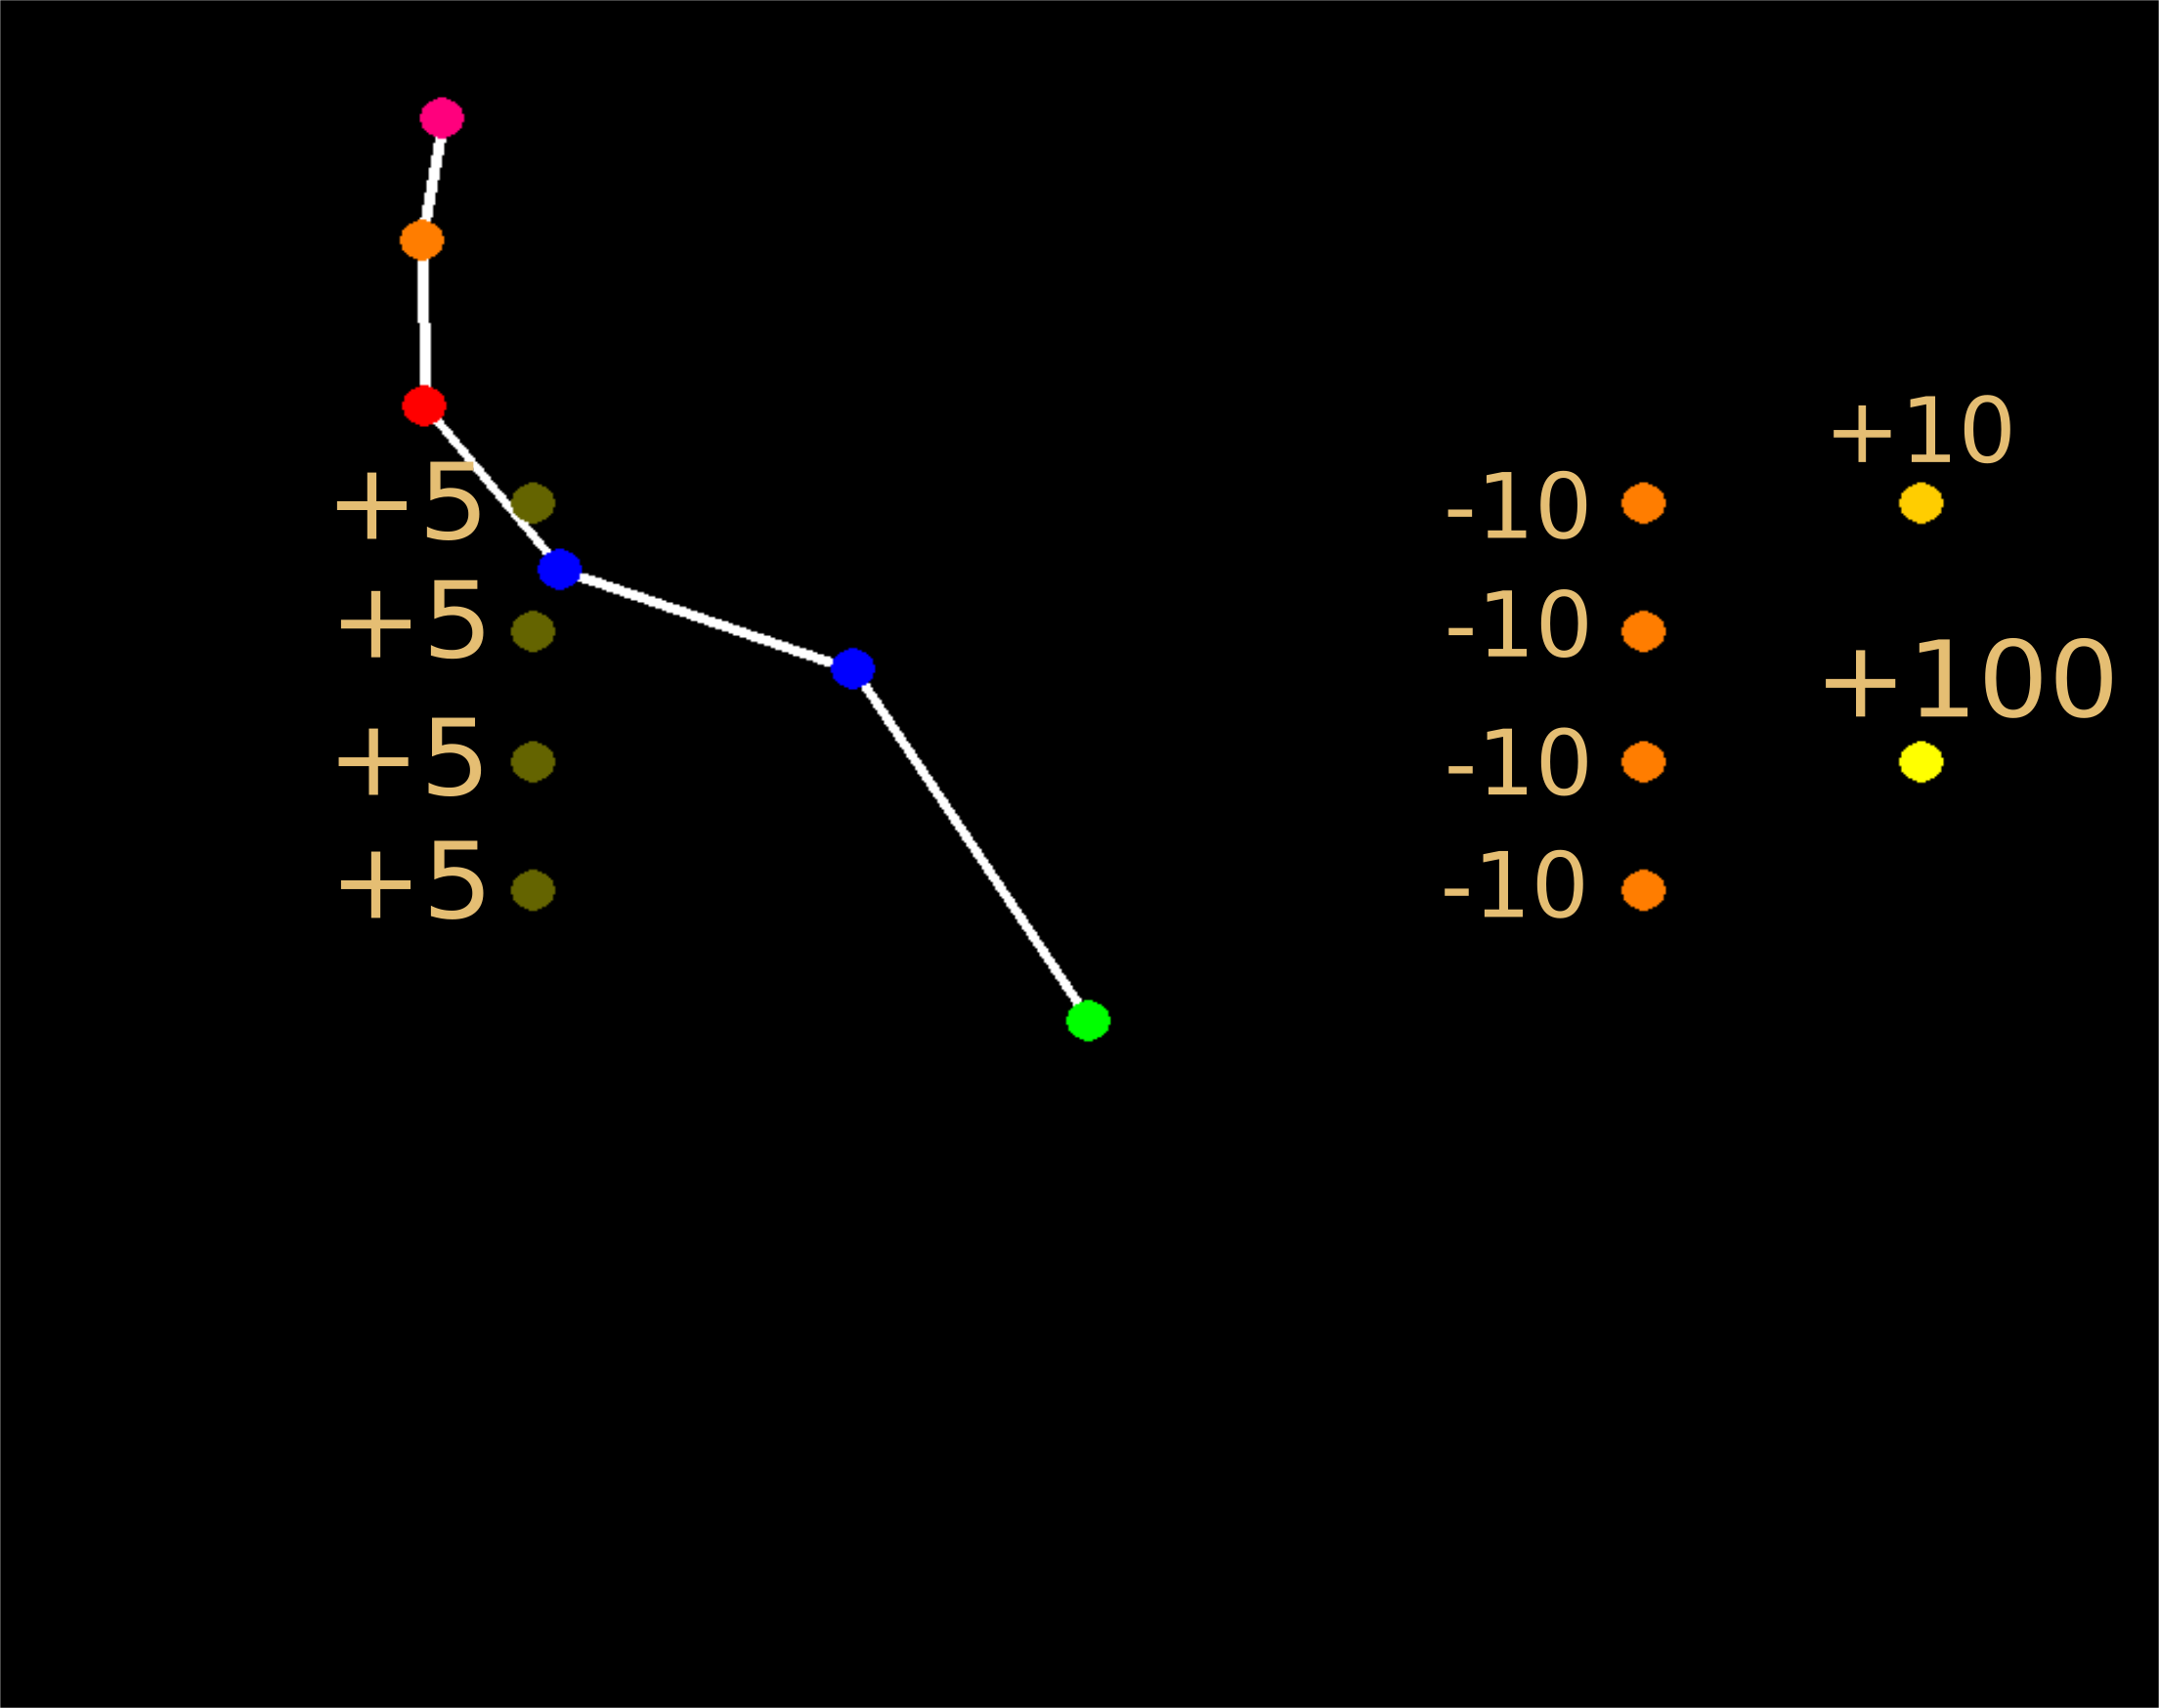
\includegraphics[scale=0.2]{img/reacher.png}
	\caption{\textit{Reacher} task with 5 joints and several reward/penalty positions}
	\label{fig:universe}
\end{figure}

\subsection{Initialized Reinforcement Learning with Supervised Learning Policy -- Policy Replacement}
Reinforcement learning algorithms usually take a long time to achieve a good policy for a specific task. And the policy always needs to be re-trained if the settings of the task are changing, even if slightly. 

There are several ways to improve the learning efficiency of reinforcement learning algorithms. One promising way is to initialize the reinforcement learning policy with a pre-trained policy. And this is especially effective when the pre-trained policy is trained on a similar task with the one the reinforcement learning is trying to solve. Moreover, if the pre-trained policy is trained across the task space containing all possible settings of a specific task that the RL is solving, it can leverage the learning performance of RL for all tasks defined in this task space.
\subsubsection{Task Specification}
In our model, we try to initialize RL with sub-optimal policy pre-trained before the RL process, and the policy is trained with supervised learning with expert trajectories sampled from inverse kinematics on \textit{Reacher} tasks. 

The task space in our model is defined to be the same `reacher' structure with one target point at different positions. The number of joints of `reacher' is chosen to be 3 with length between each pair of joints to be 200, 140 and 100, respectively. The screen size is 1000 and the fixed start point of the `reacher' is at the center of the map. The target position is sampled from a random distribution within the allowed area.
\begin{figure}[htbp]
	\centering
	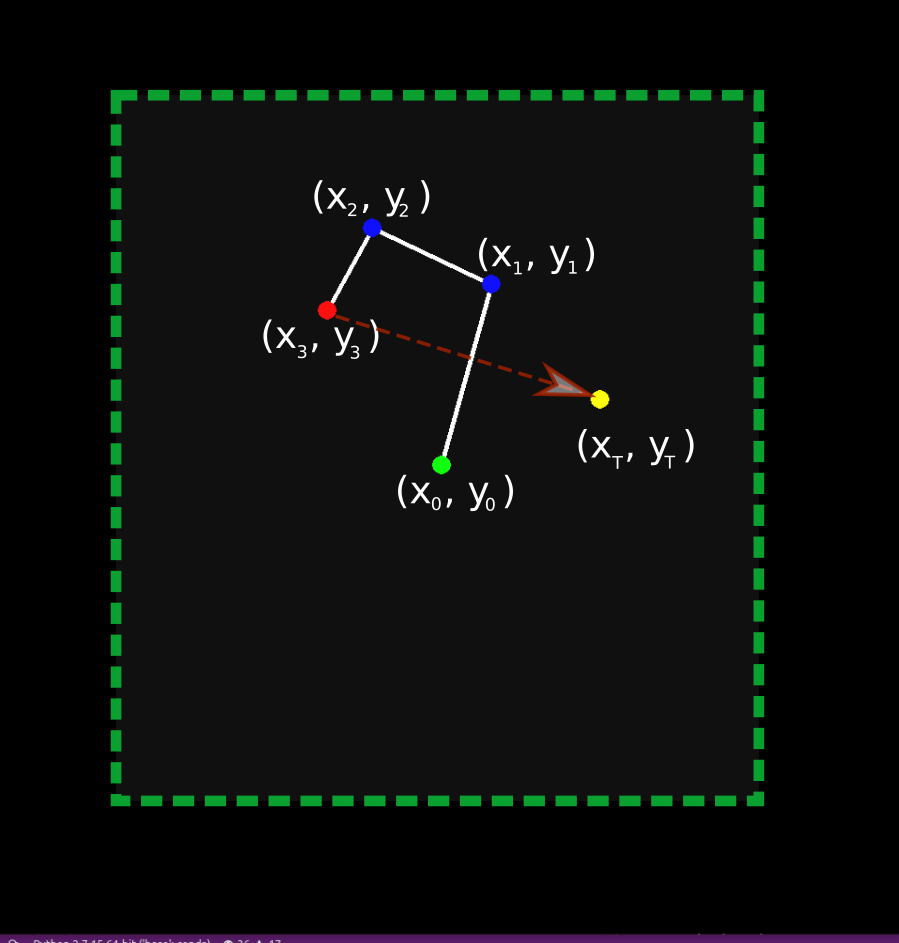
\includegraphics[scale=0.3]{img/reacher1.png}
	\caption{\textit{Reacher} task with three joints and one target point of different possible positions. The green dashed line is the area of potential target positions in the task space.}
	\label{fig:universe}
\end{figure}
The reward function for each step is defined as:
\begin{equation}
 R=\frac{R_0}{\sqrt{(x_3-x_T)^2+(y_3-y_T)^2}+1}, 
\end{equation}
where $R_0=100$ is the maximum of reward value, so $R\in(0,100]$

\subsubsection{Inverse Kinematics}
Inverse kinematics is a inverse process of forward kinematics, to derive the joint angle values with respect to the end position. Considering the end position as a transformation function of joint angels: $\mathcal{T}(\theta, L)$, where $\{\theta_i\}$ are joint angles and $\{L_i\}$ are link lengths, the forward kinematics is:
\begin{equation}
 (x_{end}, y_{end}) = \mathcal{T}(\theta, L)
\end{equation}
while the inverse kinematics needs the Jacobian of end position with respect to the joint angles parameters $\{\theta_i\}$, and to reach a specific target position $(x_T, y_T)$, the expected change of angle values are:
\begin{equation}
	(\Delta(x_{end}), \Delta(y_{end})) = \alpha (\frac{\partial(\mathcal{T}(\theta, \L))}{\partial \theta})^{-1} \cdot (x_T, y_T)
\end{equation}
where $\alpha$ is the step size. 

And in practice, we usually use Moore–Penrose pseudo-inverse for calculation of the inverse Jacobian, which will induce approximation error in trajectories.



\subsubsection{Supervised Learning Policy as Initialization}
We apply a neural network of 5 layers to train an initialization policy, with the data generated from inverse kinematics. The inputs of neural network are positions of joints and position of the target.  Each hidden layer contains 100 nodes and uses ReLu as activation function. The output layer is Tanh activated with a scaling factor of 360, to make outputs range from -360 to 360 degree as a reasonable action value of the joints. The AdamOptimizer is applied with stochastic gradient descent in the training process. The training curve is shown in Fig. 3. Note that the y-axis is transformed to be in range [-1,1] instead of [-360, 360] as the mean squared error per action value .
\begin{figure}[htbp]
	\centering
	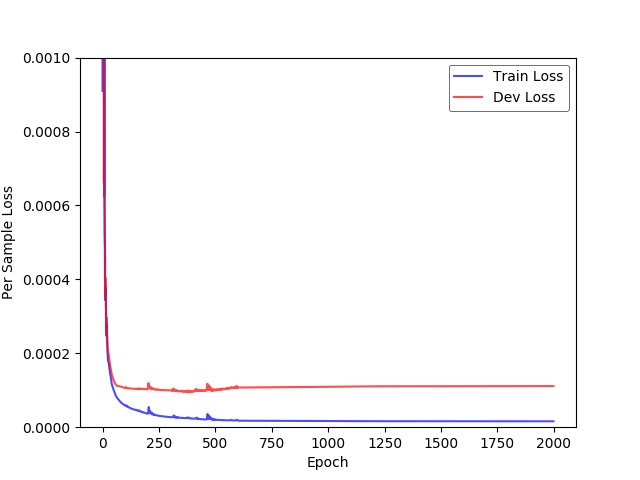
\includegraphics[scale=0.8]{img/supervised.png}
	\caption{Training curve of supervised learning with data from inverse kinematics.}
	\label{fig:universe}
\end{figure}

Here are several specifications about following experiments: (1). whenever there is a preheating process, the initial 600 steps in the learning curves are only for updating the critic (no actor update), so there is very small variance in learning curves when the noise applied is small; (2). as we are exploring the initialized policy for RL learning process, we only show experiments about the initial training steps (e.g. 2000 steps) for displaying the initialization effects.

\subsubsection{Policy Replacement}
Policy replacement is one approach to apply the policy from supervised learning in initialization of RL. The basic idea is to use the same network structure in supervised learning and the actor in RL, so that a copy can be made from the supervised learning policy to the actor as an initialization of RL. Some tricks can be applied in this process to guarantee a performance improvement, like the preheating process. 

However, potential problems exist in policy replacement approach for initialization of RL, e.g. the initialized policy is fragile in the initial training process even with small exploration noise scale, which means the initialized good policy may degrade to some worse polices (the decrease on learning curve at initial training stage) and get improved through a re-learning process. We analysed the reason for the problems and proposed some strategies for solving or alleviating it. Further analysis seen in the following subsections.

\subsubsection{DDPG with Policy Replacement -- General Process}
We apply the DDPG algorithm for the task, and show the comparisons with or without initialization for the policy.

The DDPG algorithm contains four neural networks: the actor network, the critic network, the target-actor network, and the target-critic network. For initializing the DDPG, we define the actor network and target-actor network to have exactly the same structure as the network in supervised learning. 

Initialization process of DDPG with supervised learning policy are as follows: 
(1). the weights of pre-trained supervised learning policy are loaded into the actor network and the target-actor are updated immediately; (2). samples are generated with initialized but frozen actor network with noise to pre-train the critic network; (3). train both the actor and critic network (also the target-actor and target-critic networks). Experiments show that the second step is non-trivial process for effective training DDPG with initialization. Details are explained in Sec. \ref{pretrain}.

Comparison of initial learning performances of DDPG with and without initialization policy on \textit{Reacher} task are shown in Fig. 4. The DDPG with initialization policy could significantly outperforms the one without initialization. 

\begin{figure}[htbp]
	\centering
	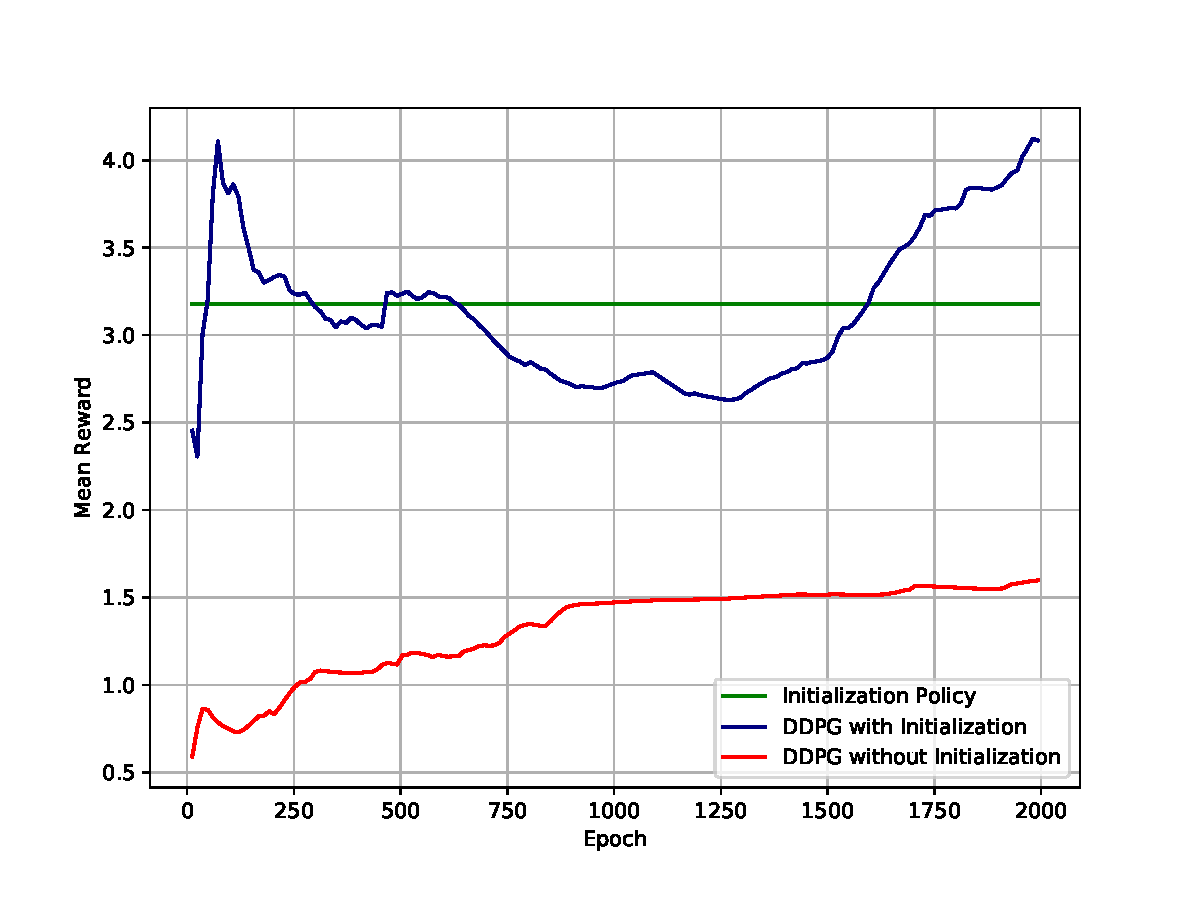
\includegraphics[scale=0.8]{img/ddpg_compare1.pdf}
	\caption{Comparison of initial learning performances of DDPG with/without initialization policy on \textit{Reacher} task. The green line is the mean reward of initial policy trained with supervised learning. The blue line and red line are mean rewards of DDPG with and without initialization in initial 2000 training epochs . }
	\label{fig:universe}
\end{figure}

There are several key components in initializing the RL with supervised learning policy affecting the performance of initialized RL (DDPG), including the scale of action noise in initialized RL, different ways of normalization in supervised learning and RL, learning rates of the actor and the critic in initialized RL, number of steps of single episode and so on. Improper settings of all above factors will affect the initialization policy to be effective for RL process. Some general intuitions about making the initialization more effective for RL are like: ensuring the inputs and outputs of the replaced policy from initialization to be as similar as possible between the supervised learning and RL, therefore applying the same input and output normalization to make sure they are of the same ranges of value, the same initial positions for each episode in `Reacher' and the same maximum length of single episode in supervised learning and RL, etc. 

\subsubsection{DDPG with Policy Replacement -- Choice of Noise}
Noise is an important factor for RL learning process. For initialized policy $\pi_i$ trained with expert trajectories, the optimal trajectory for the same task should be some neighboring trajectories of the initialized trajectory, which means the difference of optimal policy $\pi^*$ and $\pi_i$ should be within a small range $\Delta$,
\begin{equation}
	D_{KL}(\pi^*||\pi_i)<\Delta
\end{equation}
This can be derived easily by $(\pi^*(a^*|s_t)- \pi_i(a^*|s_t))<\delta$, where $a^*$ is the optimal action for state $s_t$. However, if we consider another initial policy $\pi'_i$ which is not as good as $\pi_i$, then $(\pi'^*(a^*|s_t)- \pi_i(a^*|s_t))<\delta'$ and $\delta'>\delta$, also we have $D_{KL}(\pi^*||\pi'_i)<\Delta'$ and $\Delta'>\Delta$. In order to handle different initialization policies like $\pi$ or $\pi'$, we need to apply different noise for a better learning performance.

Generally, a larger noise scale or larger probability to have a noise action will help worse policy $\pi'$ to have larger chances to sample an optimal action. We can testify the case of larger probability of have a noise through $\epsilon$-greedy policy, as shown in Fig. \ref{fig:noise}. The $\epsilon$-greedy policy is defined as follows:
\begin{equation}
\pi(a|s)=\left\{
\begin{aligned}
&1-\epsilon+\frac{\epsilon}{|A(s)|}, &a=a* \\
&\frac{\epsilon}{|A(s)|}, &a\neq a*
\end{aligned}
\right.
\end{equation}
In Fig. \ref{fig:noise}, the $\epsilon$-greedy policy can be regarded as a uniform distributed noise on the possible range of action value. It shows that the noise helps the initial policy to have a larger probability to sample the optimal action $a^*$, when the initial policy has a relatively large difference from the optimal policy, which is the case of $\pi'$ with the KL-divergence upper bound  $\Delta'>\Delta$. Fig. \ref{fig:noise1} shows that for the same optimal distribution and different initial distributions, same $\epsilon$ will cause different effects for noisy policy. Generally, it shows that large $\epsilon$ value (0.8) only helps with large divergence of initial policy and optimal policy. And this is the reason to apply decayed $\epsilon$ in practice for $\epsilon$-greedy policy.

Fig. \ref{fig:noise2} shows that when two policies have large divergence $\Delta'$, larger $\epsilon$ in will help more for the initial policy to sample optimal actions with $\epsilon$-greedy policy. And larger $\epsilon$ generally means larger chances to have noisy actions.
\begin{figure}[htbp]
	\centering
	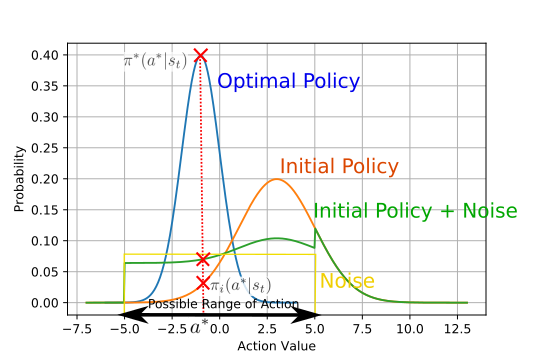
\includegraphics[scale=0.8]{img/noise2.png}
	\caption{A figure showing why adding noise would help for exploring better actions, with noise type of $\epsilon$-greedy policy. Suppose the initial policy and the optimal policy are Gaussian distributions with different means and variances, and the noise is a uniform distribution within specific range (range of possible action value). The figure shows how the noise of $\epsilon$-greedy helps to increase the possibility for non-optimal policy to sample the optimal action }
	\label{fig:noise}
\end{figure}

\begin{figure}[htbp]
	\centering
	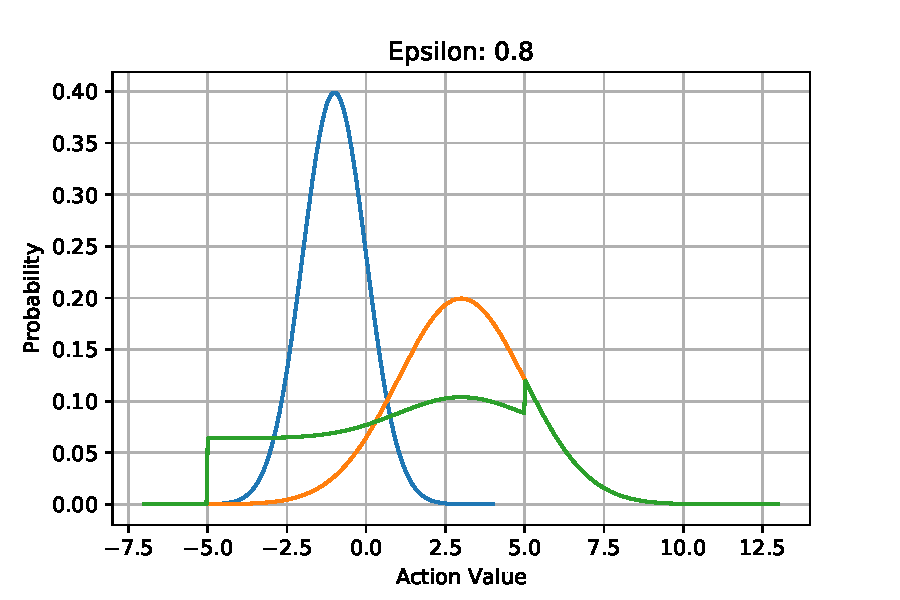
\includegraphics[scale=0.4]{img/noise28.pdf}
	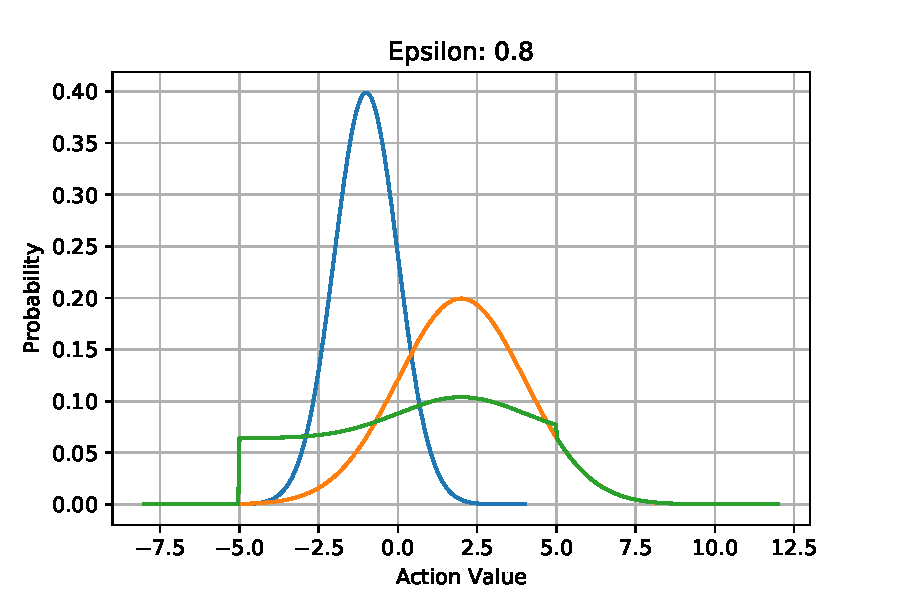
\includegraphics[scale=0.4]{img/noise38.pdf}
	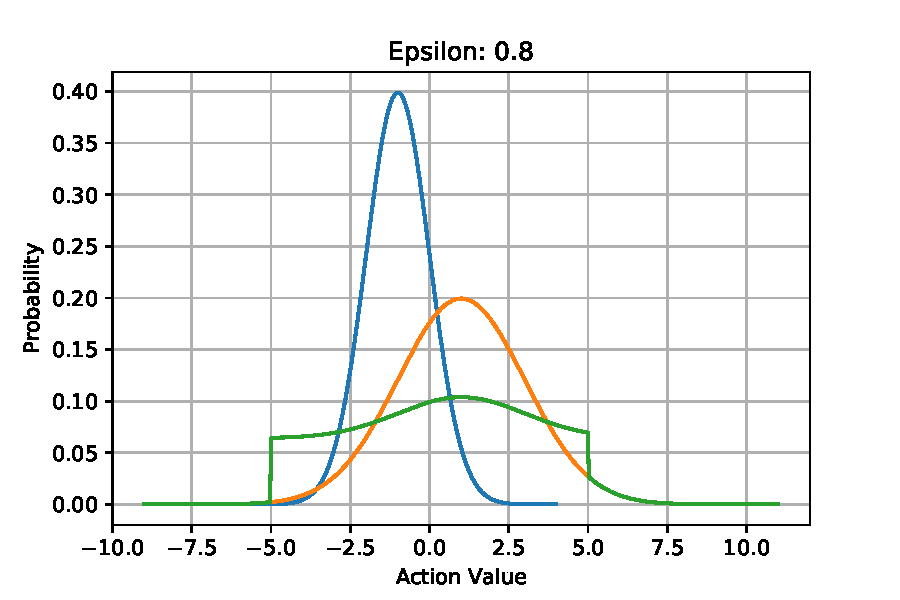
\includegraphics[scale=0.4]{img/noise48.pdf}
	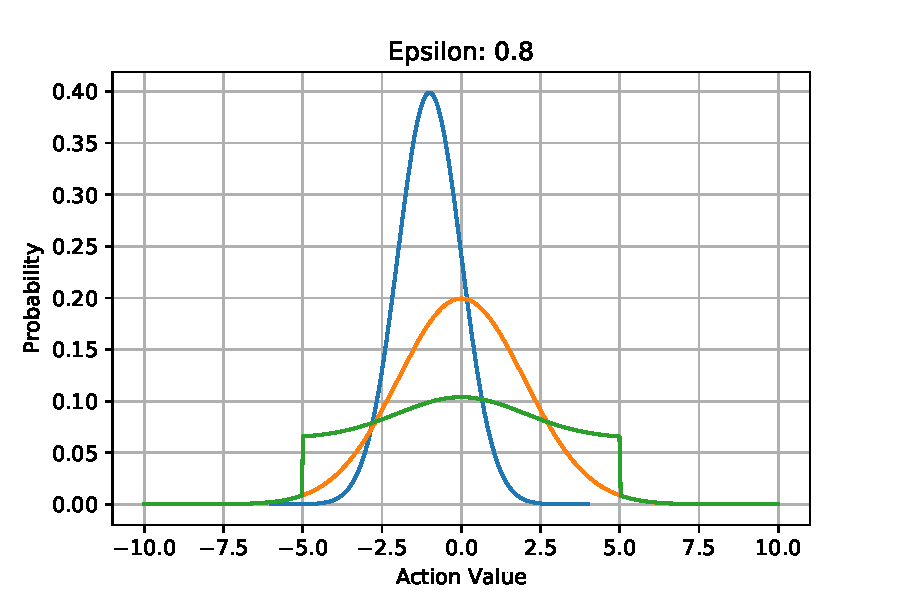
\includegraphics[scale=0.4]{img/noise58.pdf}
	\caption{$\epsilon$-greedy policy with different initial distributions and same $\epsilon$ value. It shows the same $\epsilon$ will cause different effects for noisy policy, it benefits the top two initial distribution and hurts the bottom two distributions. So large $\epsilon$ value (0.8) only helps with large divergence of initial policy and optimal policy. }
	\label{fig:noise1}
\end{figure}

\begin{figure}[htbp]
	\centering
	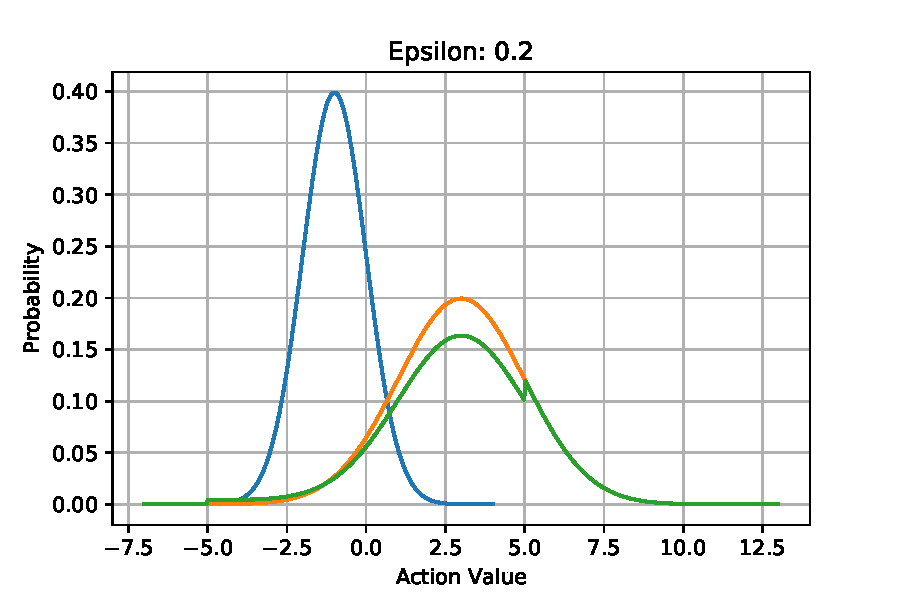
\includegraphics[scale=0.4]{img/noise22.pdf}
	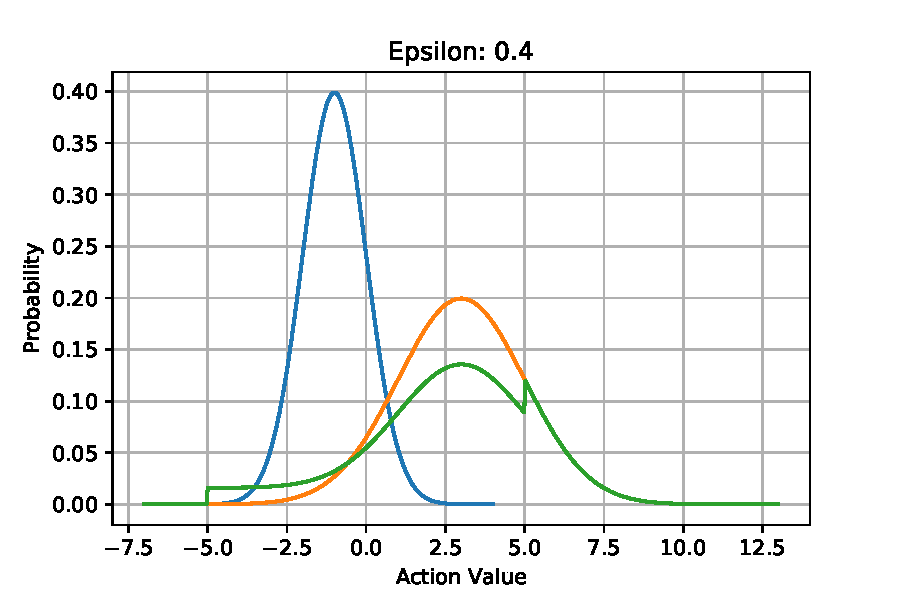
\includegraphics[scale=0.4]{img/noise24.pdf}
	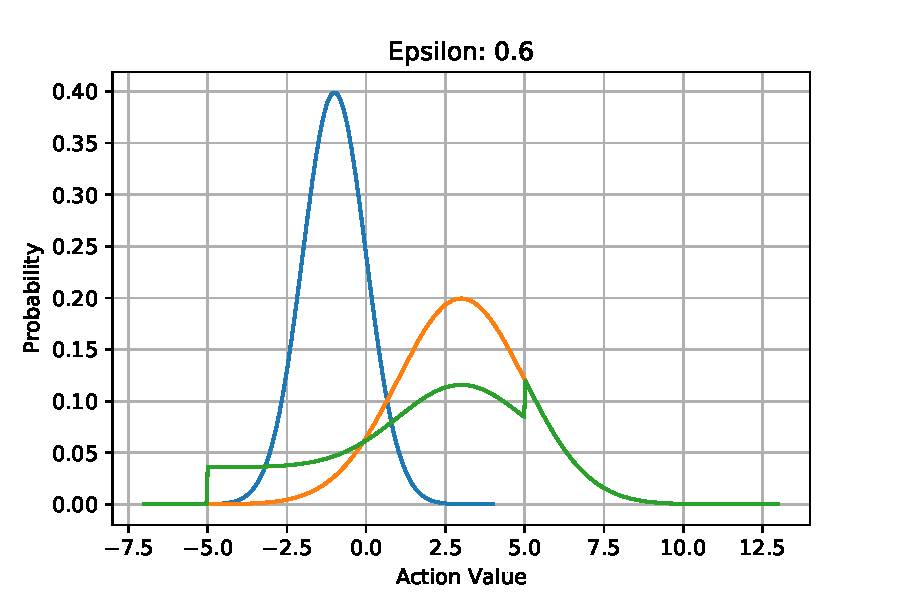
\includegraphics[scale=0.4]{img/noise26.pdf}
	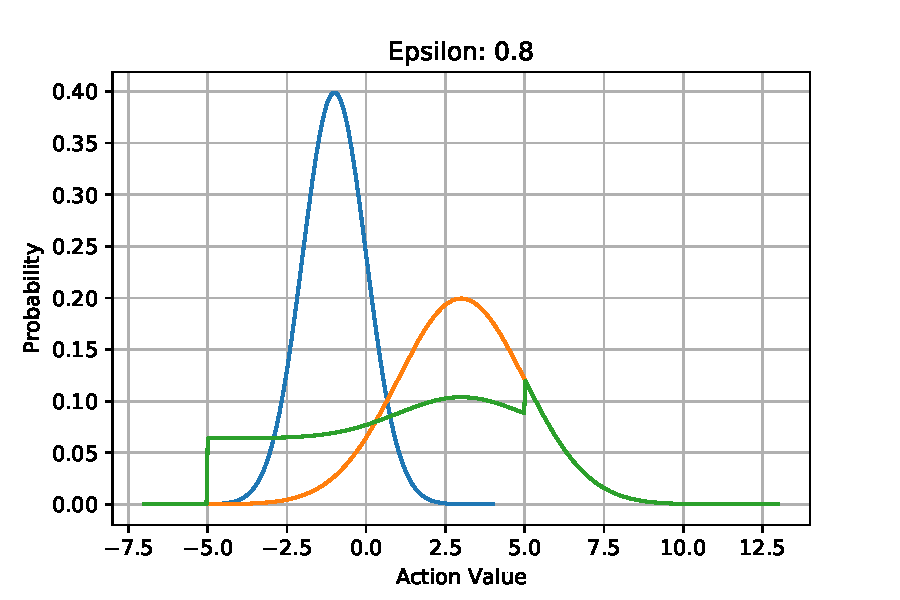
\includegraphics[scale=0.4]{img/noise28.pdf}
	\caption{$\epsilon$-greedy policy with different $\epsilon$ value and same initial and same optimal distribution. Larger $\epsilon$ value benefits more for large divergence between the optimal policy and the initial policy. }
	\label{fig:noise2}
\end{figure}
Above analysis is based on $\epsilon$-greedy policy, which represents the variety of probability to apply the noise in actions. However, the case of the variety in scale of noise has similar effects for different distributions. Therefore, we can derive some conclusions that for better initial policy, it means the smaller the divergence it is from the optimal policy, therefore it needs to apply noise with a smaller probability or apply smaller scale noise. So, how does it work in initialized RL?

In initialized RL, the cases are the same. Experiments with different initialized policy for DDPG on \textit{Reacher} task are shown in Fig. \ref{fig:noise3}, in which the relatively good initial policy $\pi$ is called from expert, and the relatively bad but better than random initial policy $\pi'$ is called the half-expert. Fig. \ref{fig:noise3} shows that for a bad initial policy, which has a relatively large divergence from the optimal policy, larger noise scale works better for improving the learning performance. And this results testify the above analysis of the case of $\epsilon$-greedy policy. Note that the experiments shown in Fig. \ref{fig:noise3} are all without preheating process, which is the second step described in the general process section. However, if we take experiments on the policy initialized from a better policy, Fig. \ref{fig:noise4} shows smaller noise is better for DDPG initialized with an expert policy, which also testifies above analysis results.
\begin{figure}[htbp]
	\centering
	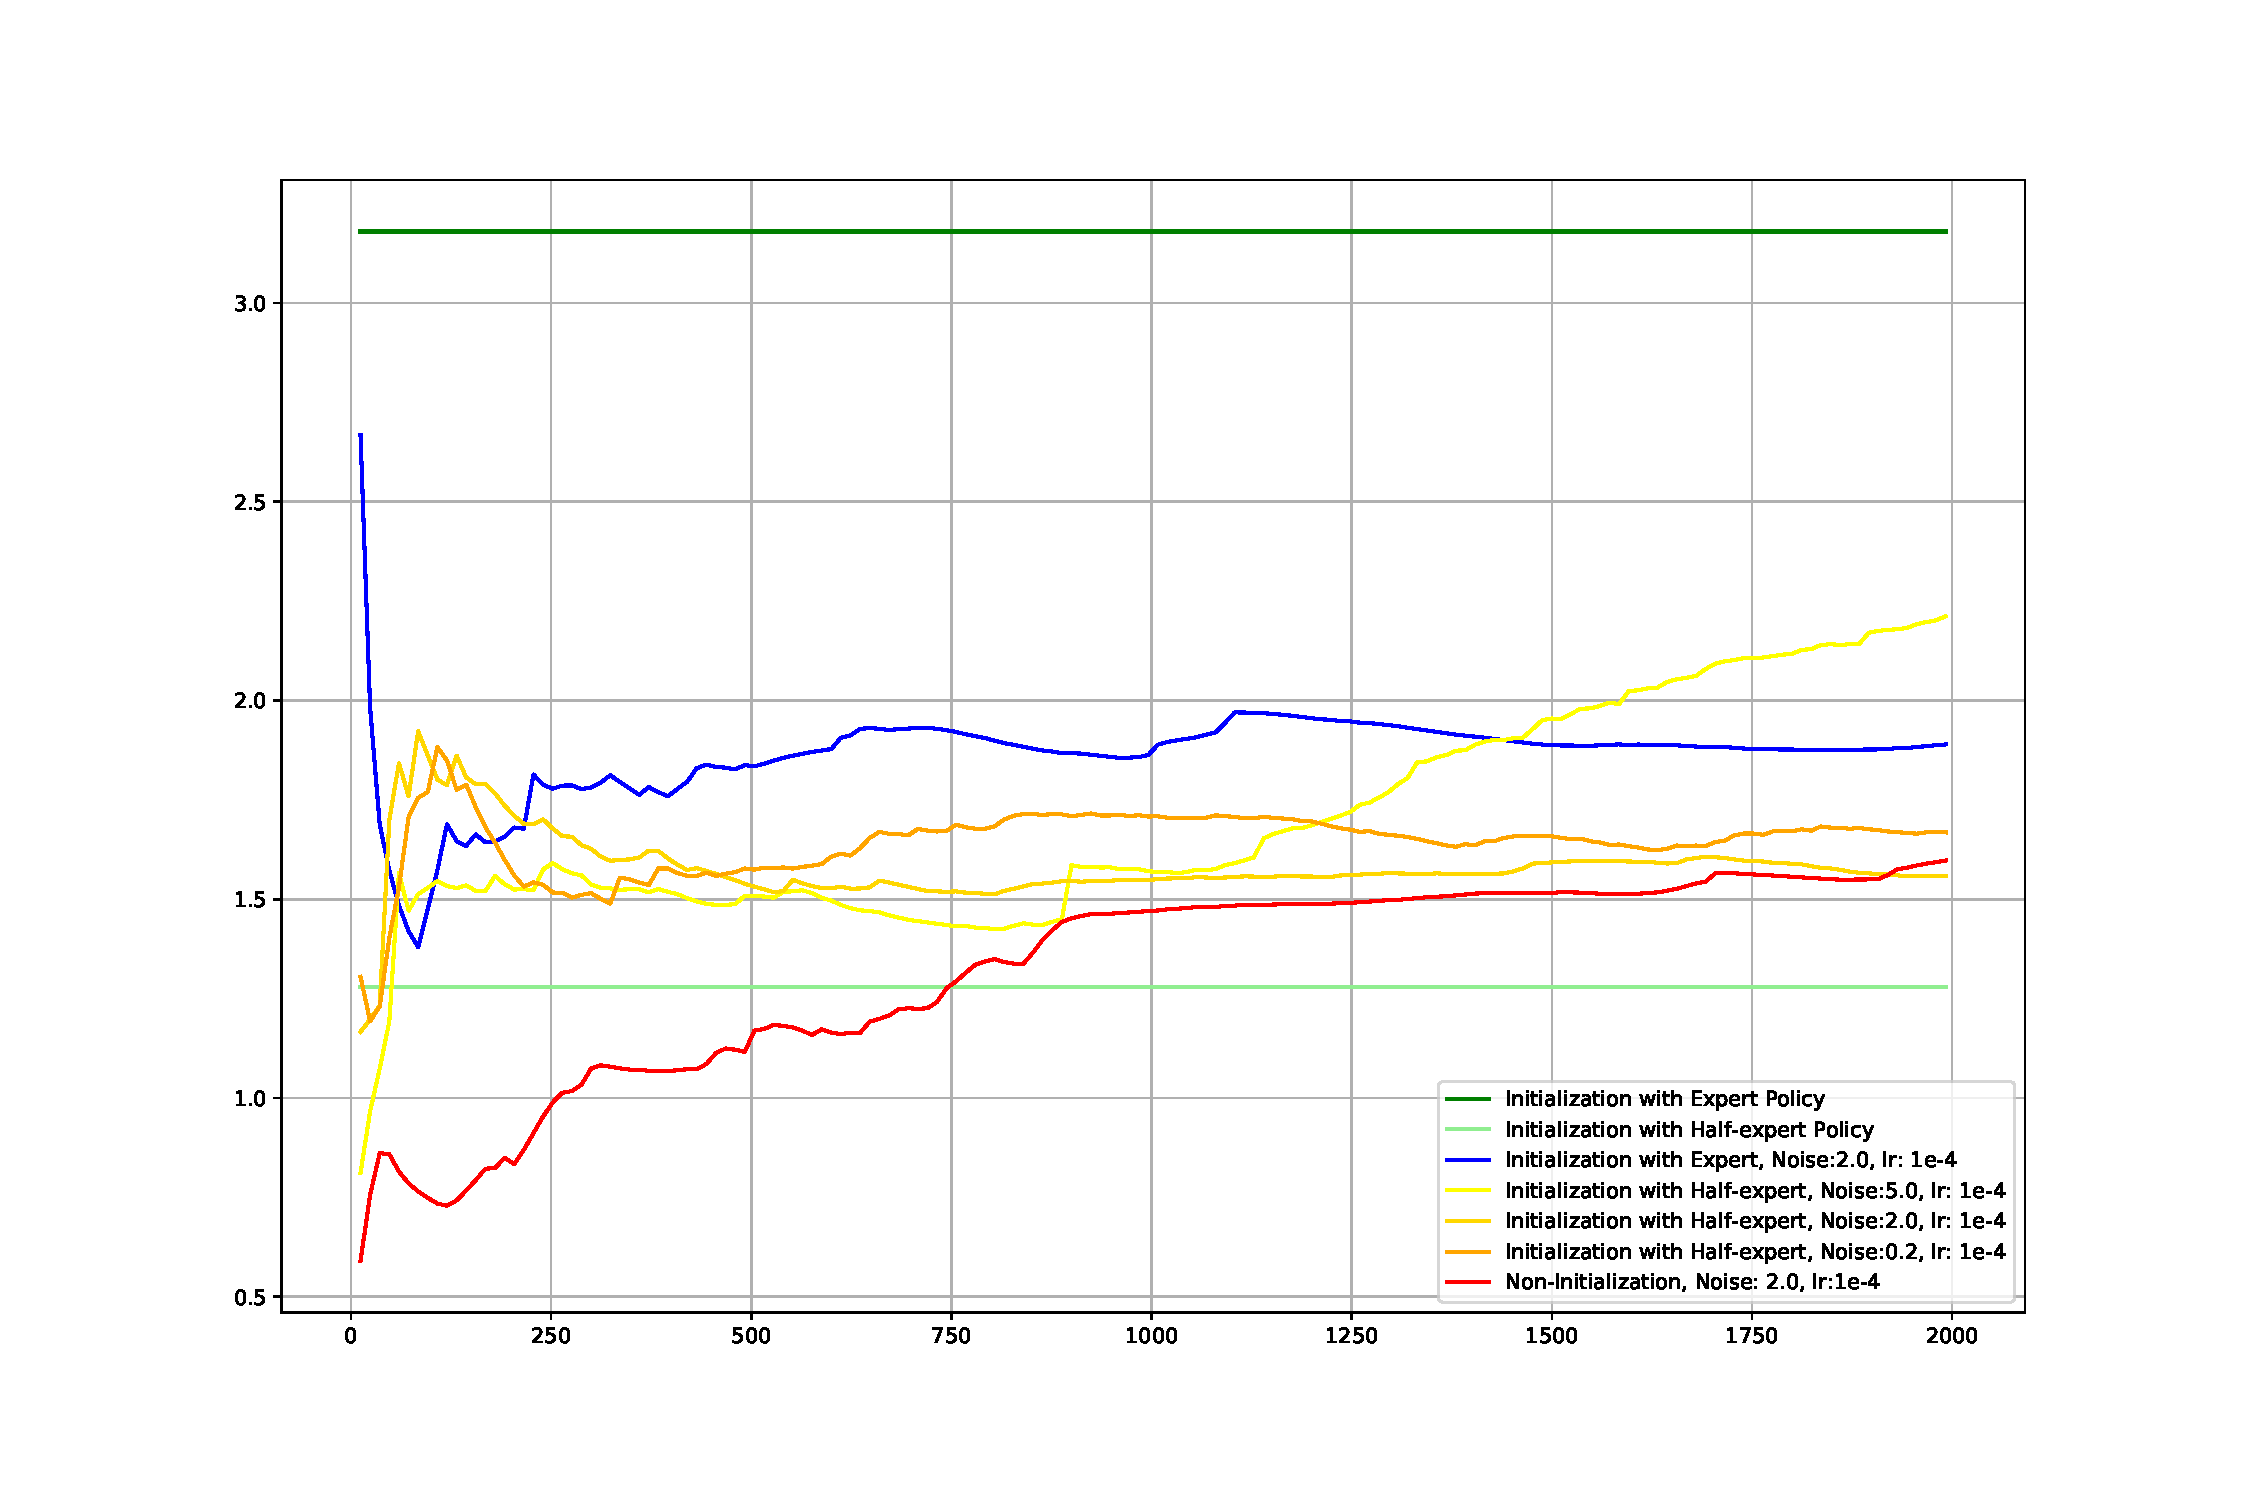
\includegraphics[scale=0.4]{img/ddpg_compare3.pdf}
	\caption{Experiments with different initialized policy for DDPG on \textit{Reacher} task}
	\label{fig:noise3}
\end{figure}

\begin{figure}[htbp]
	\centering
	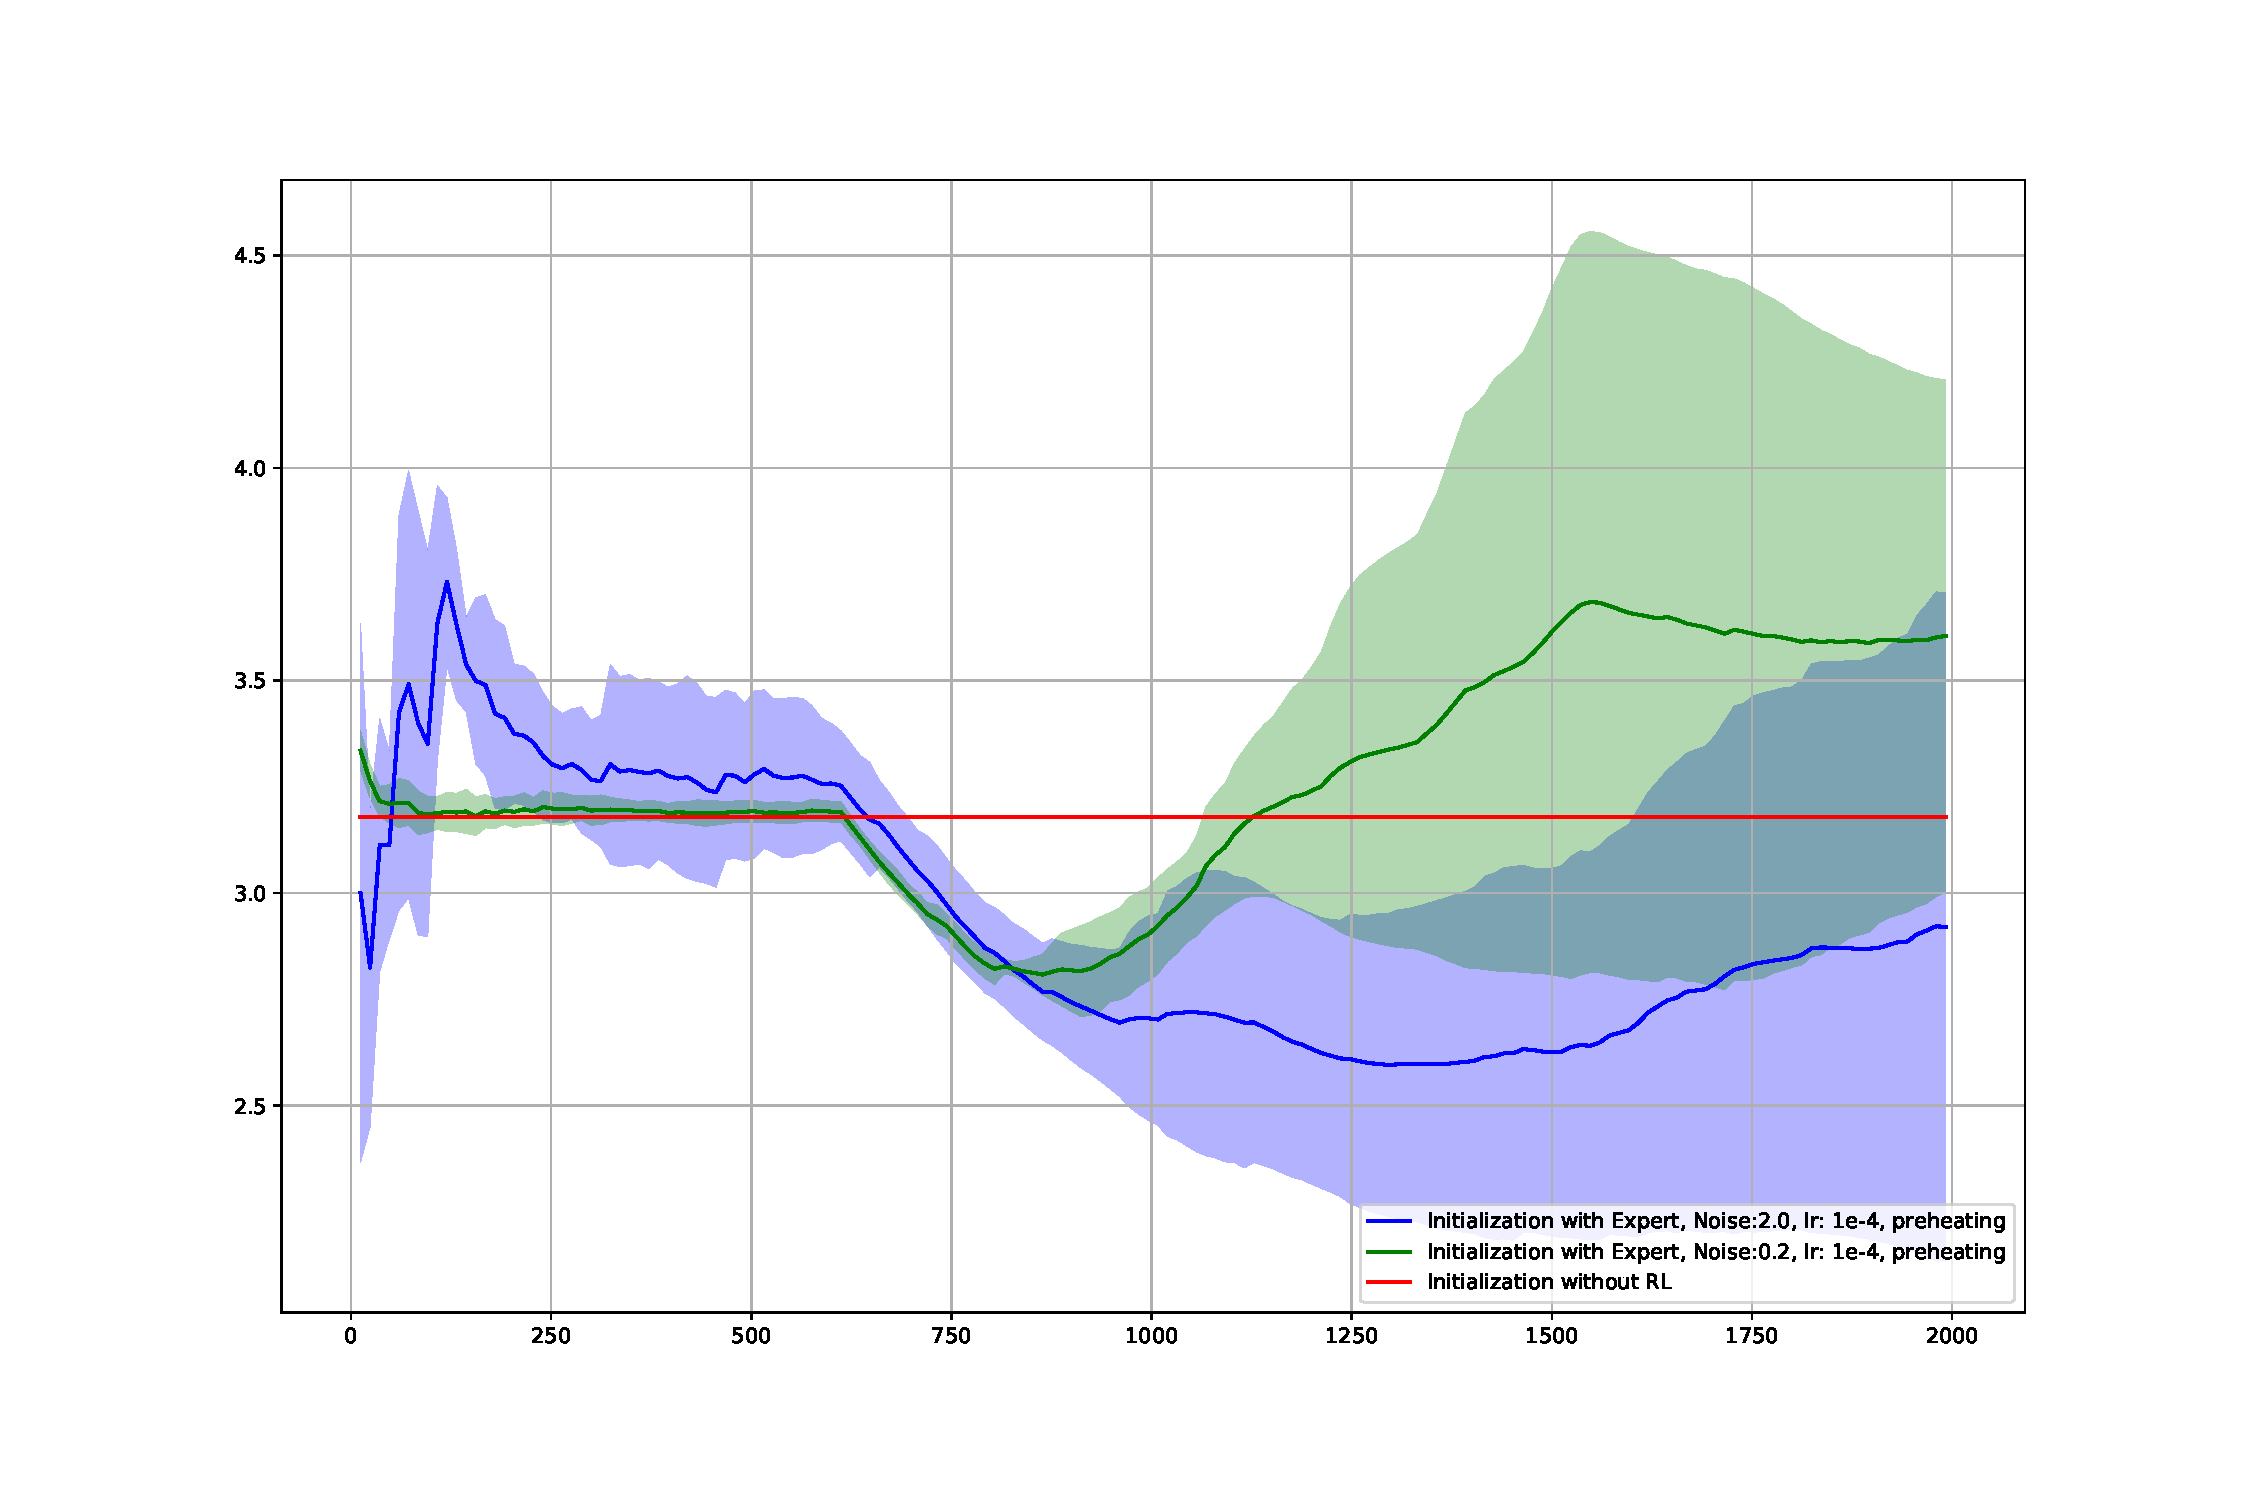
\includegraphics[scale=0.4]{img/ddpg_compare4.pdf}
	\caption{Experiments with different initialized policy for DDPG on \textit{Reacher} task}
	\label{fig:noise4}
\end{figure}

\begin{figure}[htbp]
	\centering
	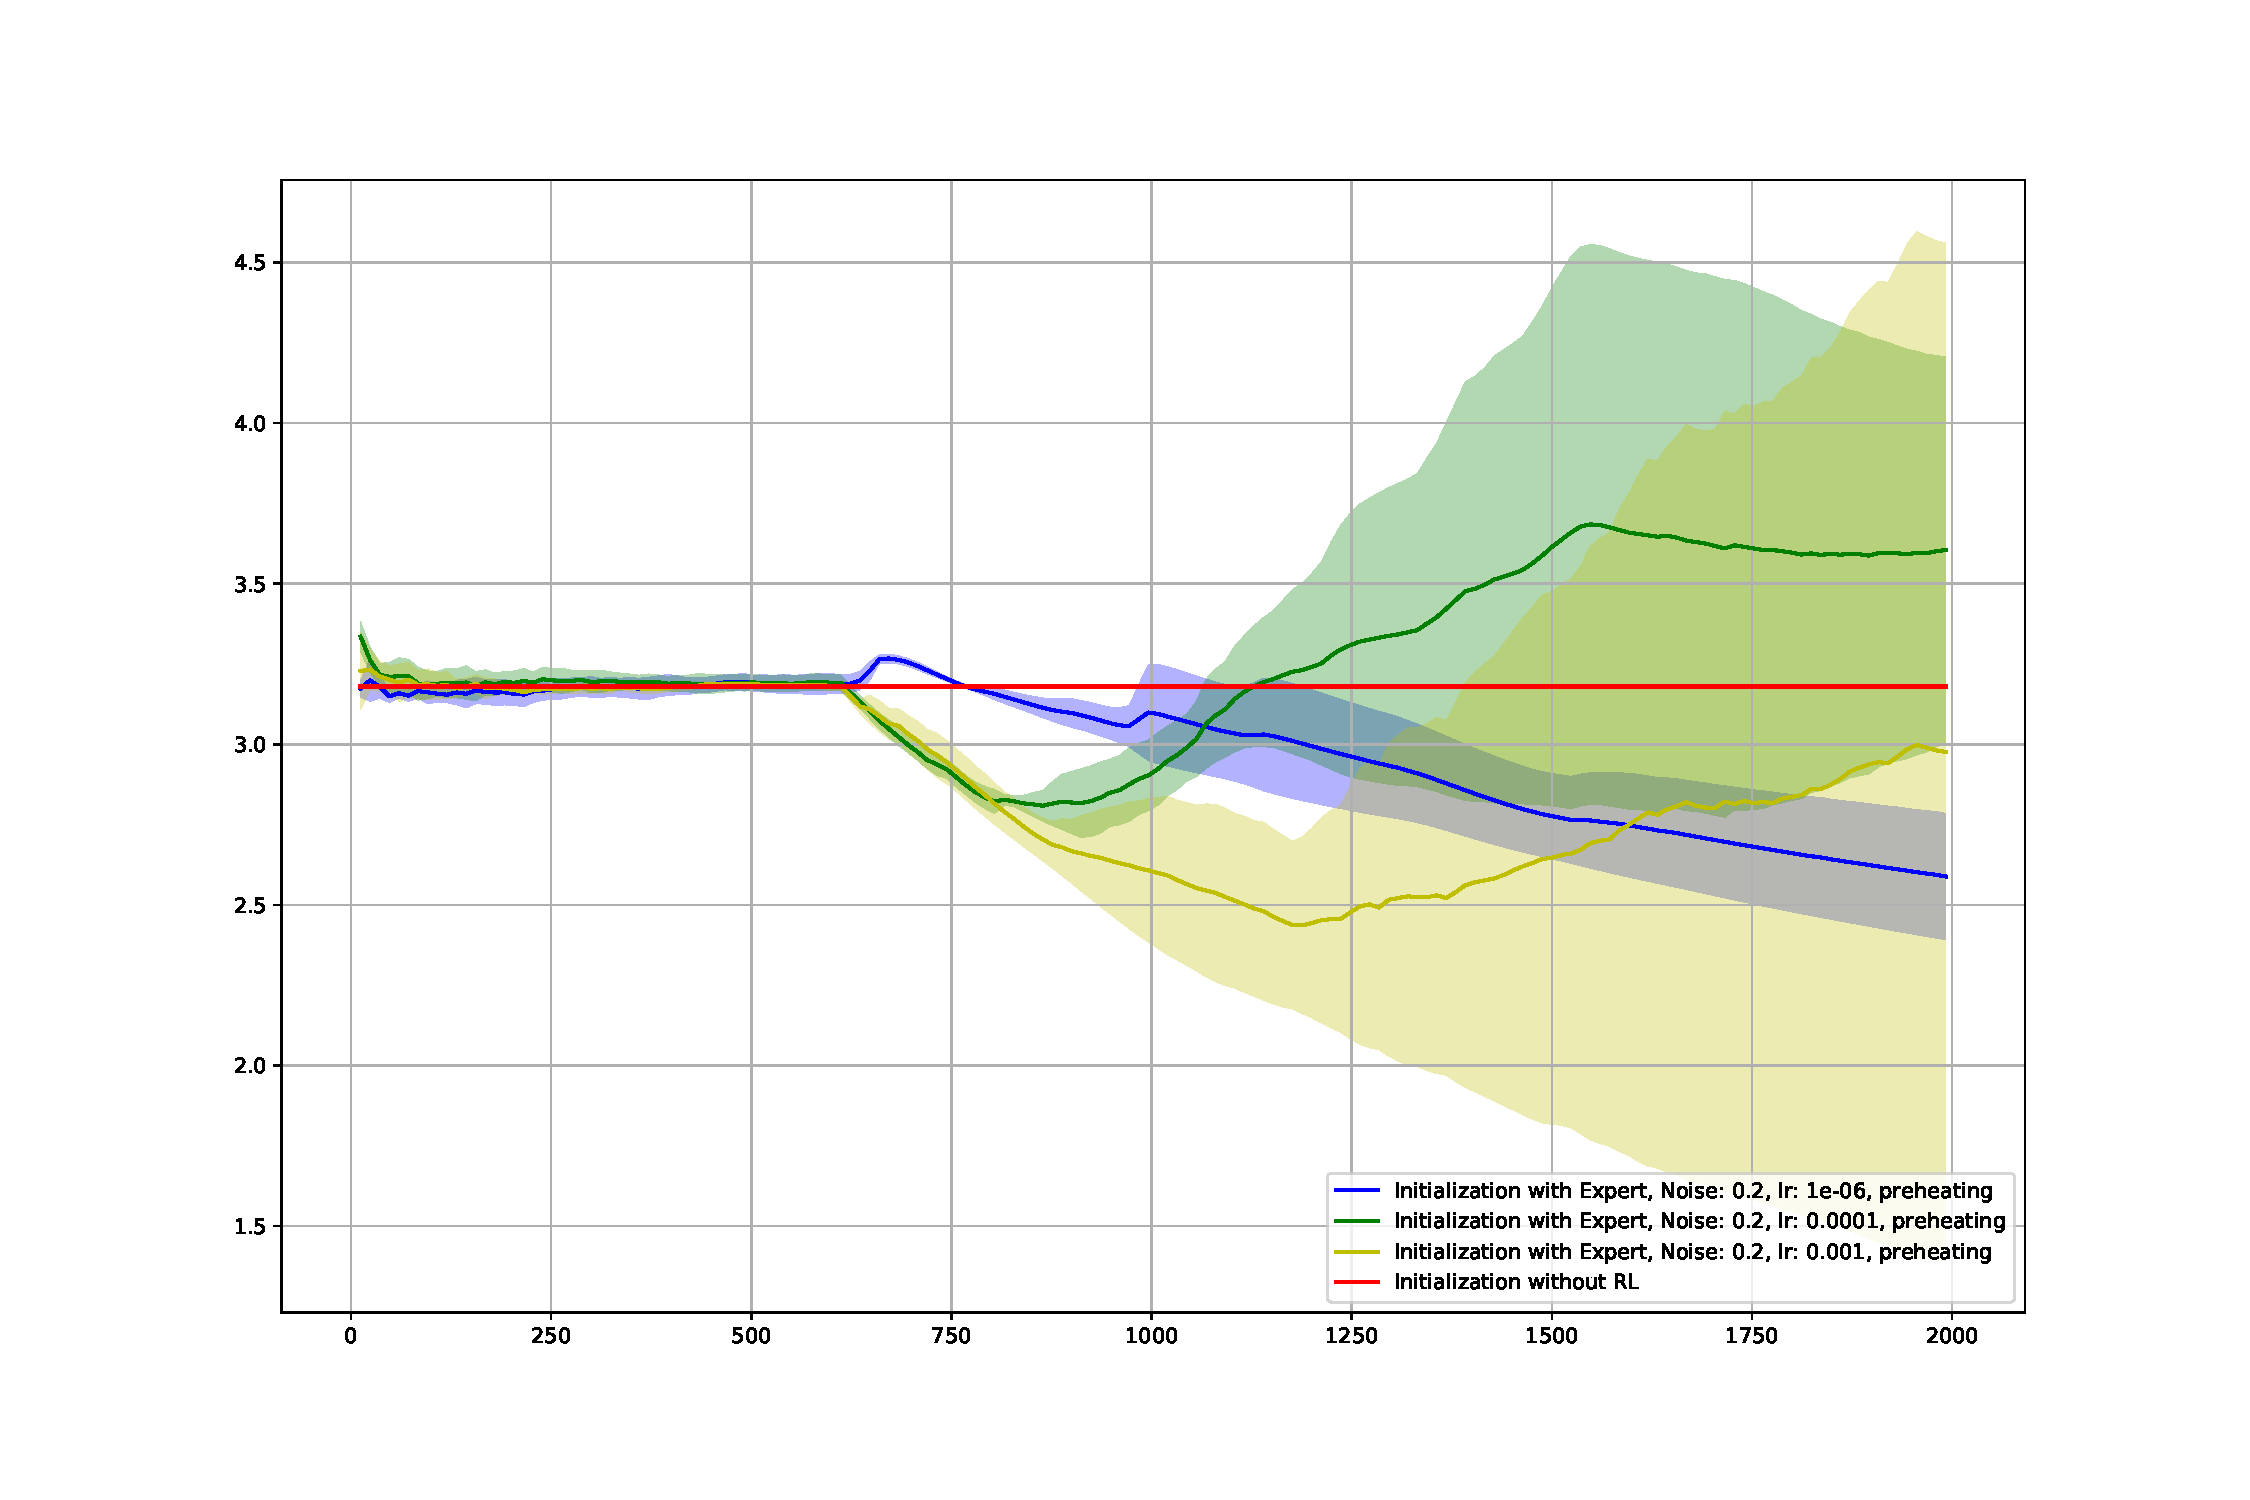
\includegraphics[scale=0.4]{img/ddpg_compare5.pdf}
	\caption{Experiments with different initialized policy for DDPG on \textit{Reacher} task}
	\label{fig:noise5}
\end{figure}

As for the learning rate settings, Fig. \ref{fig:noise5} shows a comparison of different actor learning rate for initialized DDPG with a proper noise scale. For initialized DDPG from an expert policy, we actually need only tune the parameters in the actor neural networks in a small range, which requires a small scale of actor learning rate (e.g. $10^{-4}$). A larger learning rate could change the networks dramatically and also the outputs. However, when the actor learning rate is too small, it will not help with learning process as shown in Fig. \ref{fig:noise5}.


\subsubsection{DDPG with Policy Replacement -- Pre-train the Critic}\label{pretrain}
The actor-critic scheme is important in DDPG, as the critic instructs the actor's choise of action values through evaluating the Q-value of each action. Therefore, a good critic is critical for the DDPG to show great learning performance in a task. However, in initialized policy for RL, the supervised learning with inverse kinematics could only mapping from the input states to the output actions, without any reference of the estimated value of each action. It means the critic of DDPG cannot be directly initialized with policy from supervised learning. Therefore, the role of the critic is amplified in the learning process of initialized DDPG, which is testified in experiments of this section. To solve the problem that the supervised learning policy can only initialized the actor networks, we propose a pre-training process of the critic in initialized DDPG called the 'preheating', with which the initialized policy could be more effective than without it.

The `preheating' process is conducted as follows: after loading the weights from pre-trained policy to the actor networks in DDPG, we sample from the frozen actor to generate near-expert samples with noise scale $\sigma$ and feed them into the memory (DDPG is off-policy learning), then train the critic networks with generated samples for $N_{pre}$ epochs. The frozen actor can be achieved through setting the actor learning rate to be 0 in practice. After the `preheating' step of $N_{pre}$ epochs, we train the initialized DDPG in a general way. 

As shown in Fig. \ref{fig:pretrain}, without pre-training the critic, there is always a severely decrease in performances of the initialized DDPG algorithm, no matter what the scale of exploration noise is. The decrease phenomenon for initialized DDPG without preheating can be explained as follows: the main problem of initialized policy for RL without preheating is that the virtue of initialized policy is ruined too quickly through changing of the weights of the initialized actor, and this is always the case as long as the learning rate is of a relatively considerable value. Because no matter how much the exploration noise is, the weights of the actor will be changed according to the learning rate of the actor, and neural network as an estimator has property of sensitivity on weights, which ends up with a dramatic changing in output policy of the actor. Therefore the actor will diverge fast from the initial near-expert policy, without a good critic. A good critic means it shows positive instructions for the actor to update weights in the correct direction. On the other hand, a good actor here in initialized DDPG will have great chances to decrease its performance with a random initialized critic. Therefore the `pre-heating' process actually prevent the actor from updating to hurt the performances, or at least alleviate it. This is shown clearly in Fig. \ref{fig:pretrain} that the lower bound of initialized DDPG with preheating is much higher than without the preheating process.
\begin{figure}[htbp]
	\centering
	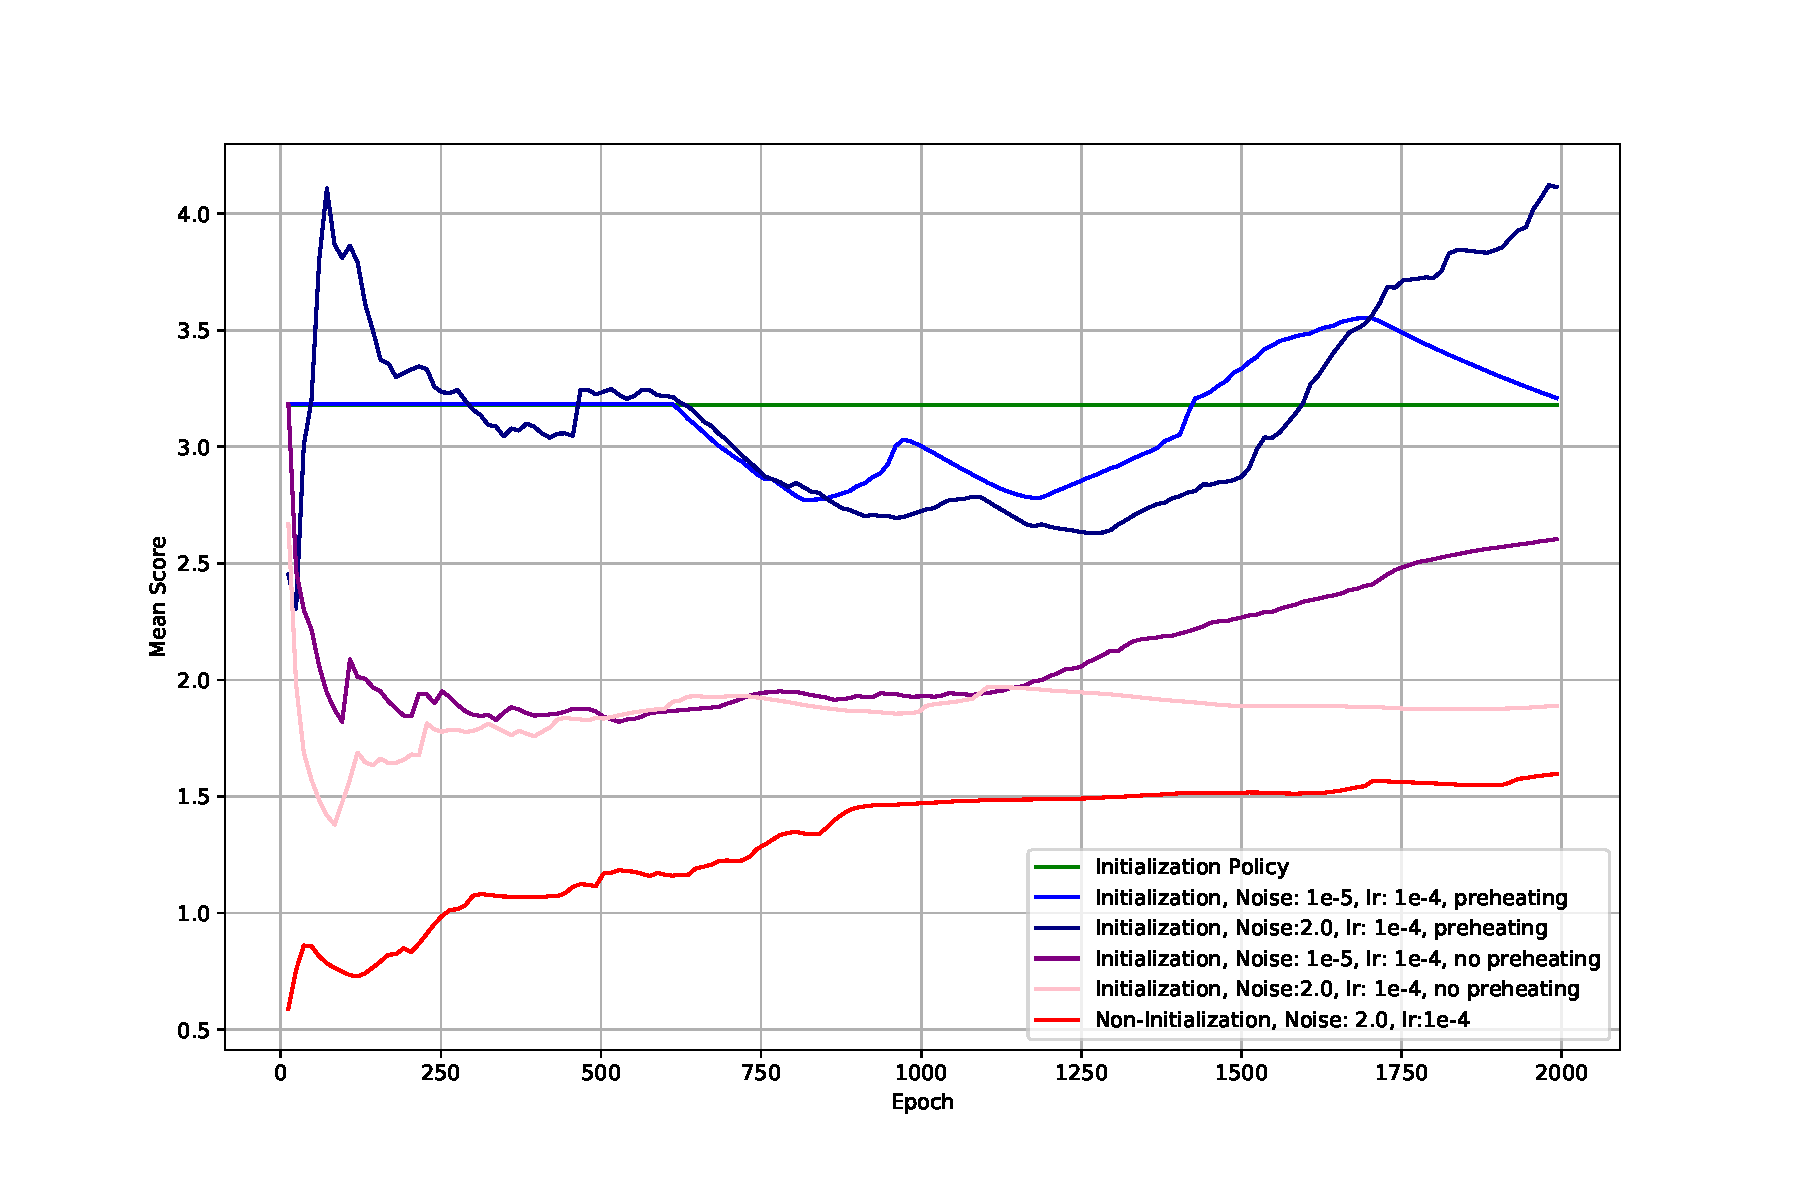
\includegraphics[scale=0.5]{img/ddpg_compare2.pdf}
	\caption{Comparison of initialized DDPG with/without pre-training the critic on \textit{Reacher} task. The green line is the mean reward of initial policy trained with supervised learning.}
	\label{fig:pretrain}
\end{figure}

\subsubsection{DDPG with Policy Replacement -- Conclusions}
Some conclusions can be derived from above analysis and experiments about DDPG with initialization policy for \textit{Reacher} task:
(1). Different initial policy requires different noise scales to achieve better performances. For expert initialization policy, smaller exploration noise for DDPG shows better learning effects; for half-expert initialization policy, larger noise shows better learning effects.

(2). The preheating process is important for initialized policy on DDPG: with the pre-training of the critic before general learning process of DDPG, the learning performance is always better than without it, It reduces the dramatic decrease at the initial training phase when the DDPG is initialized with an expert policy. The important intuition from this is that we should not use the critic for instructing the actor unless it's good enough for a good actor.


\subsubsection{PPO with Policy Replacement}
PPO is an on-policy RL algorithm, and its exploration is controlled by the variance $\sigma$ of output action distribution from the policy neural network, which is learned during the training process. We can control the scale of exploration through adding a value to the variance, which is called noise base $\sigma_0$ here. So the actual action variance is $\sigma =\sigma_0+\sigma_{pre}$ where $\sigma_{pre}$ is trained output variance of the policy network.

The preheating process for PPO is conducted by pre-training the value evaluation network, similar to pre-training the actor in DDPG. 

Fig. \ref{fig:ppo1} shows comparisons of initialized PPO for \textit{Reacher} task. Similar to conclusions in initialized DDPG algorithm, the preheating process is effective for reducing the decrease in initial training phase of PPO when initialized from an expert policy.
\begin{figure}[htbp]
	\centering
	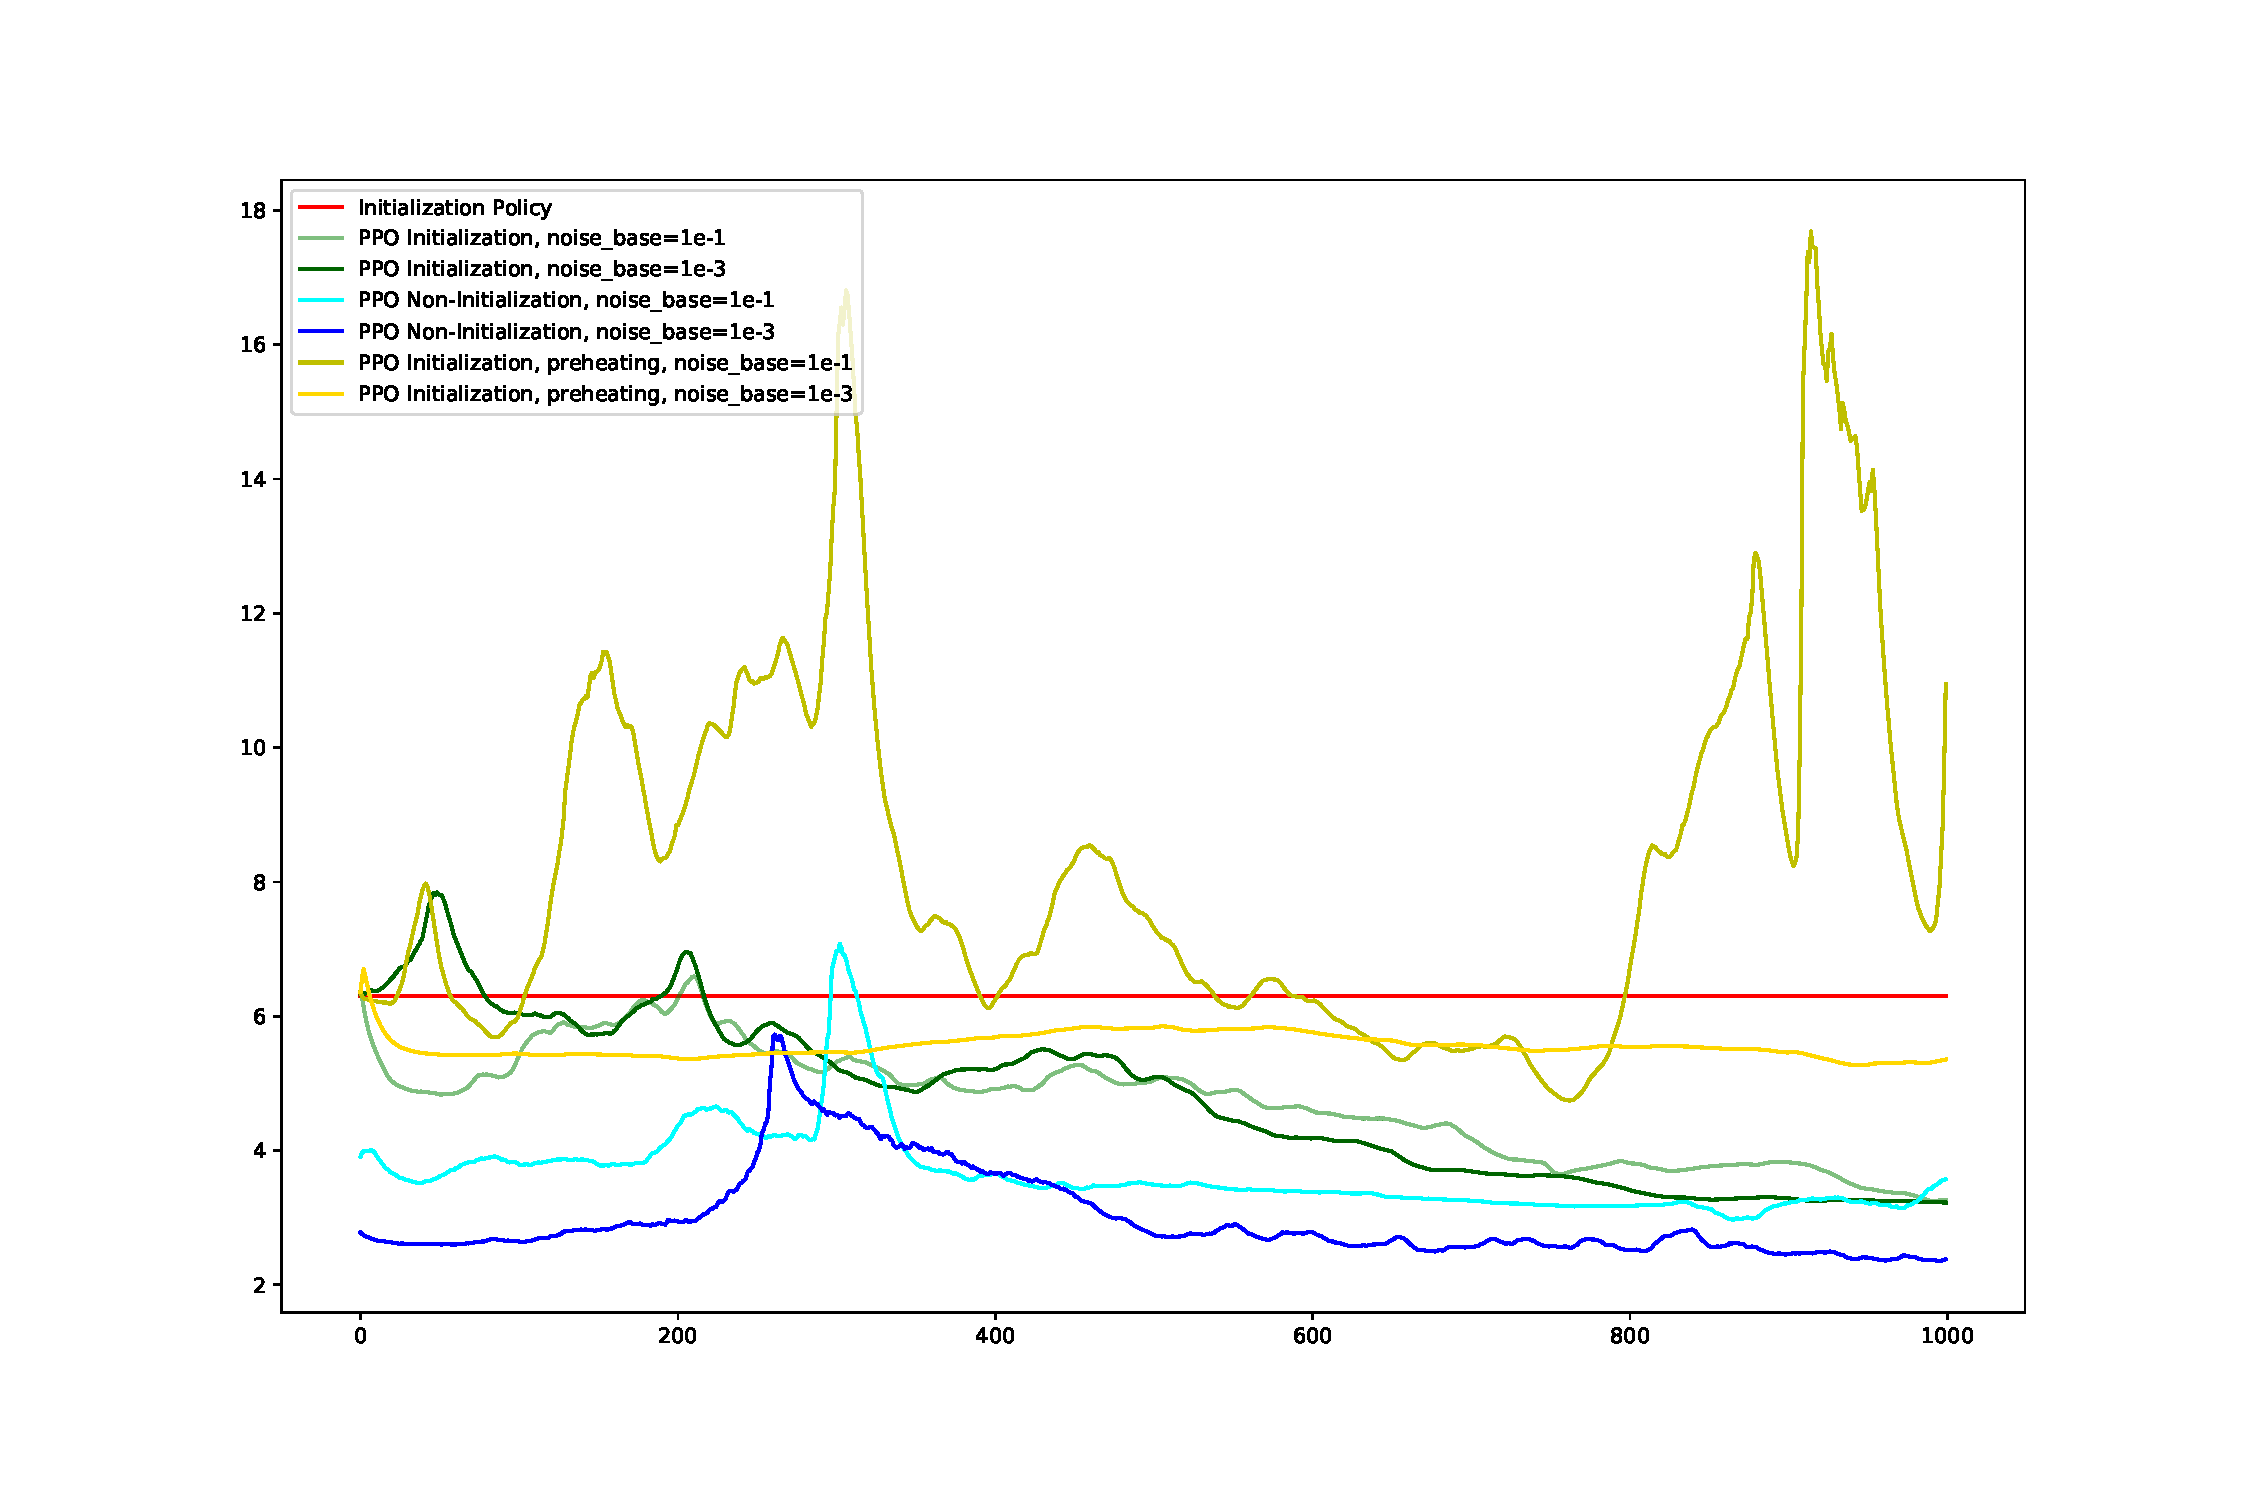
\includegraphics[scale=0.4]{img/ppo_compare2.pdf}
	\caption{Comparisons of PPO with or without initialized policy and preheating process with different noise scale.}
	\label{fig:ppo1}
\end{figure}

\begin{figure}[htbp]
	\centering
	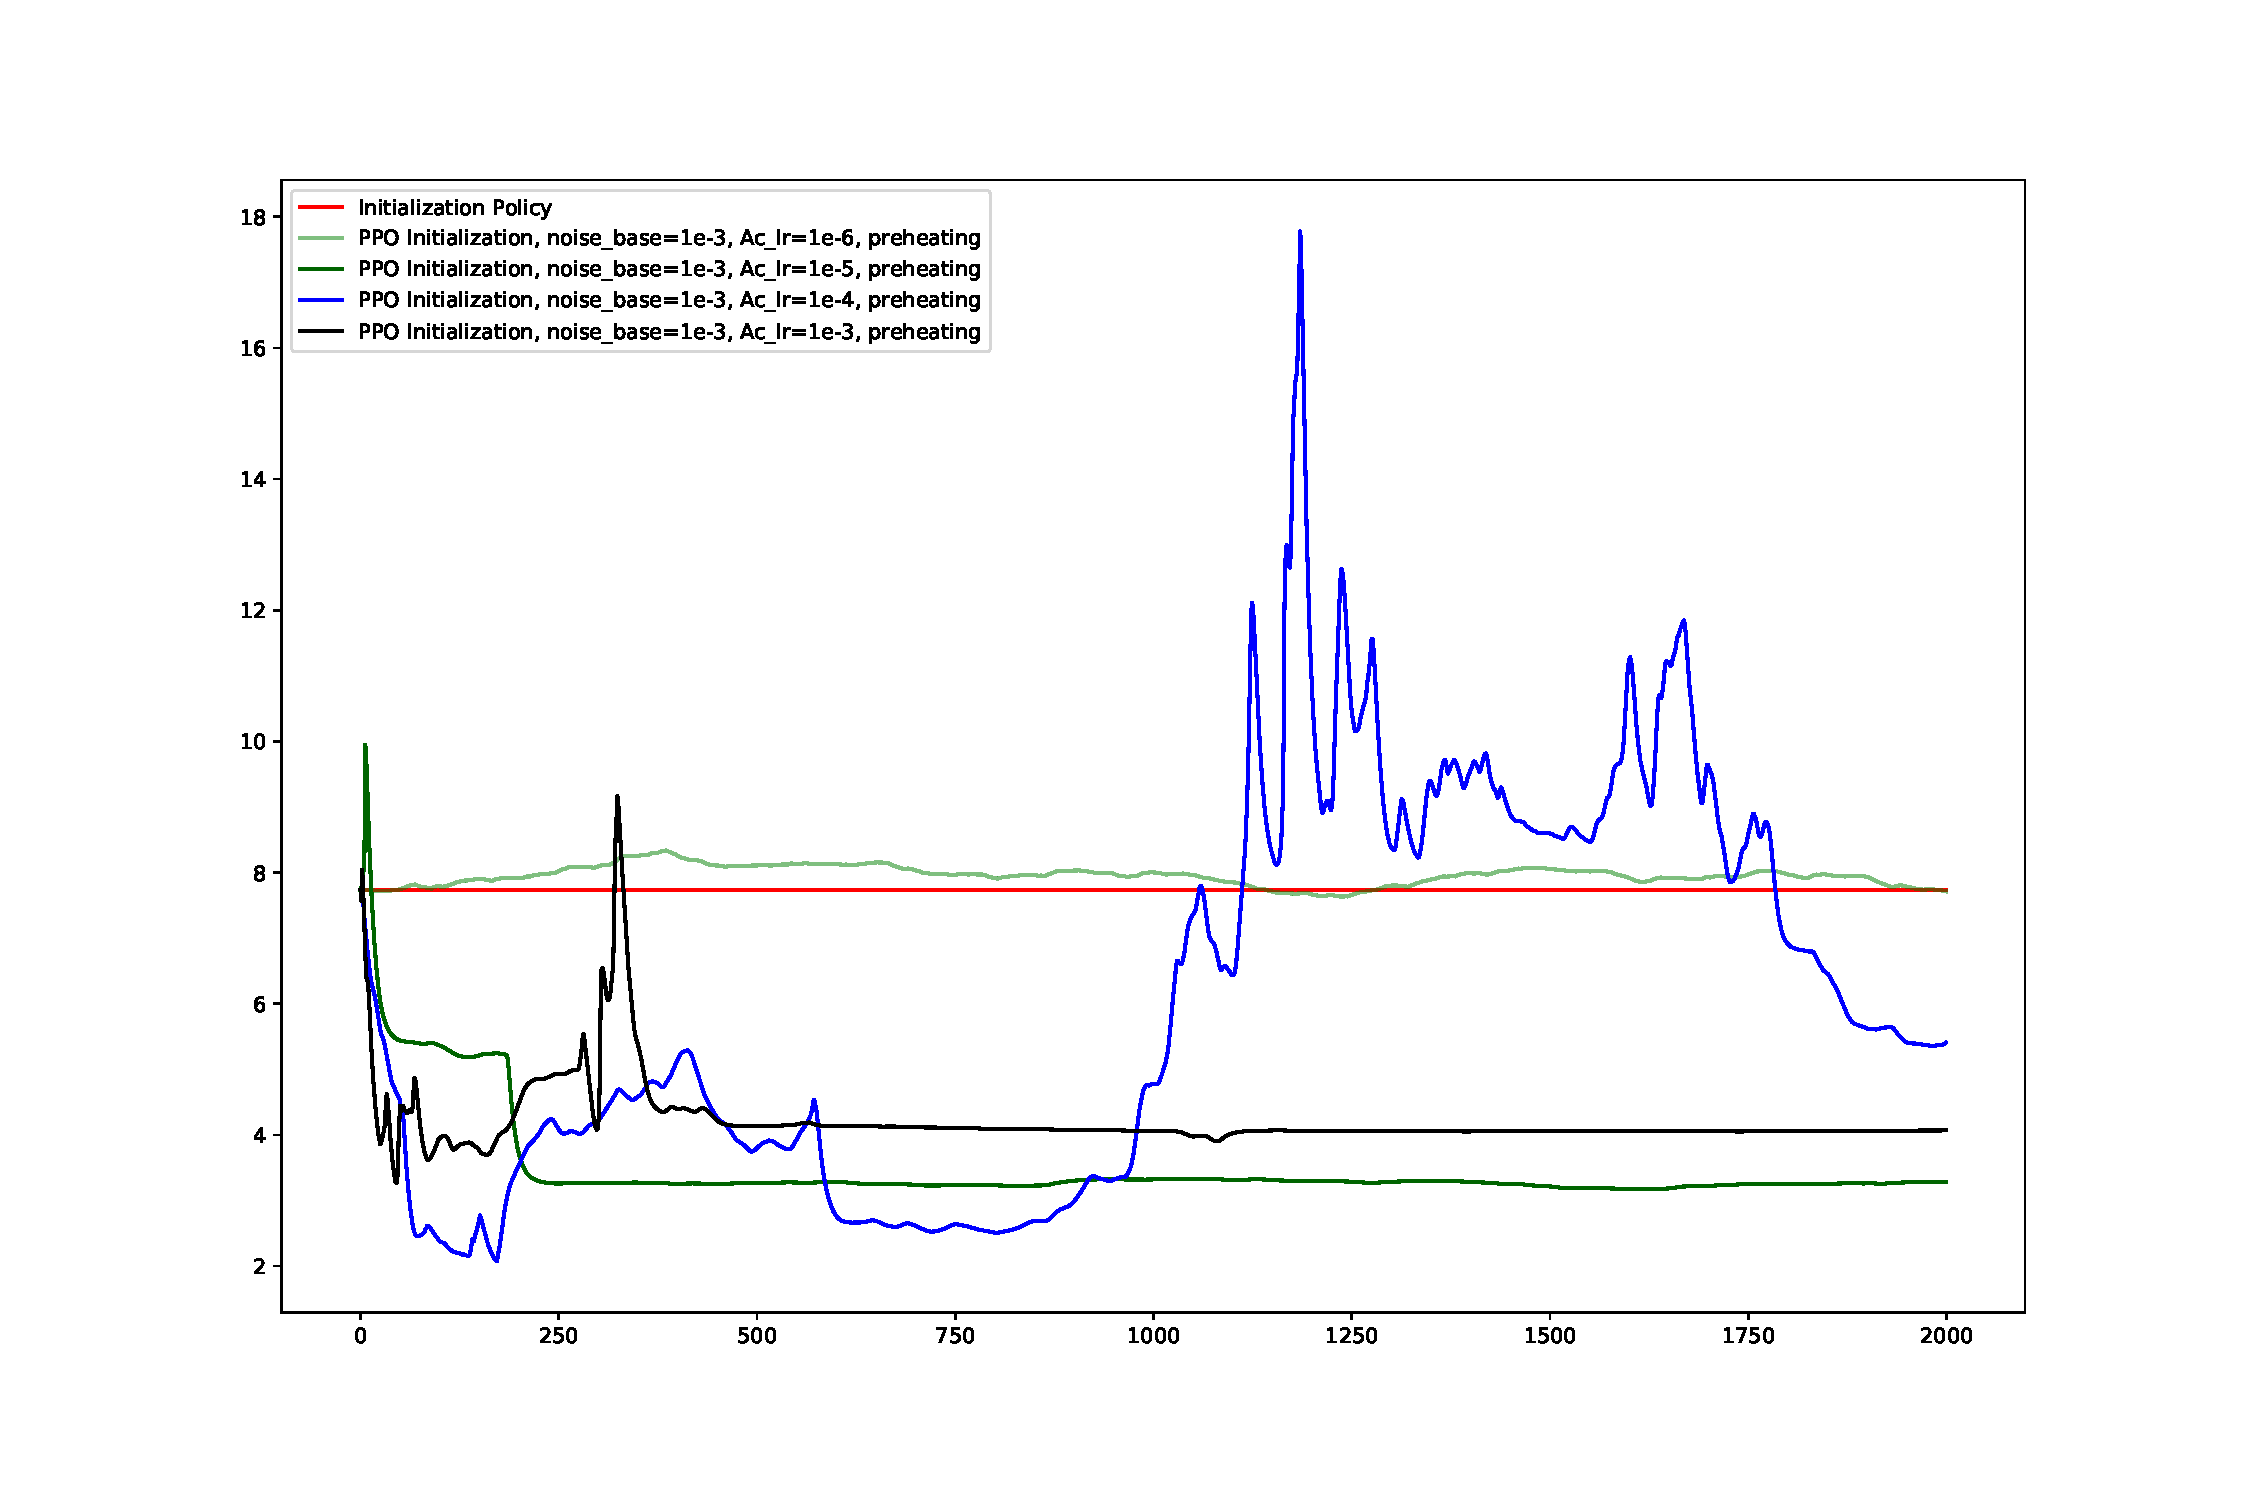
\includegraphics[scale=0.4]{img/ppo_compare3.pdf}
	\caption{Comparison of different actor learning rates for initialized PPO with preheating process on \textit{Reacher} task.}
	\label{fig:ppo2}
\end{figure}

Fig. \ref{fig:ppo2} shows different actor learning rates for initialized PPO. A proper range of actor learning rate is needed for effective learning.

\begin{figure}[htbp]
	\centering
	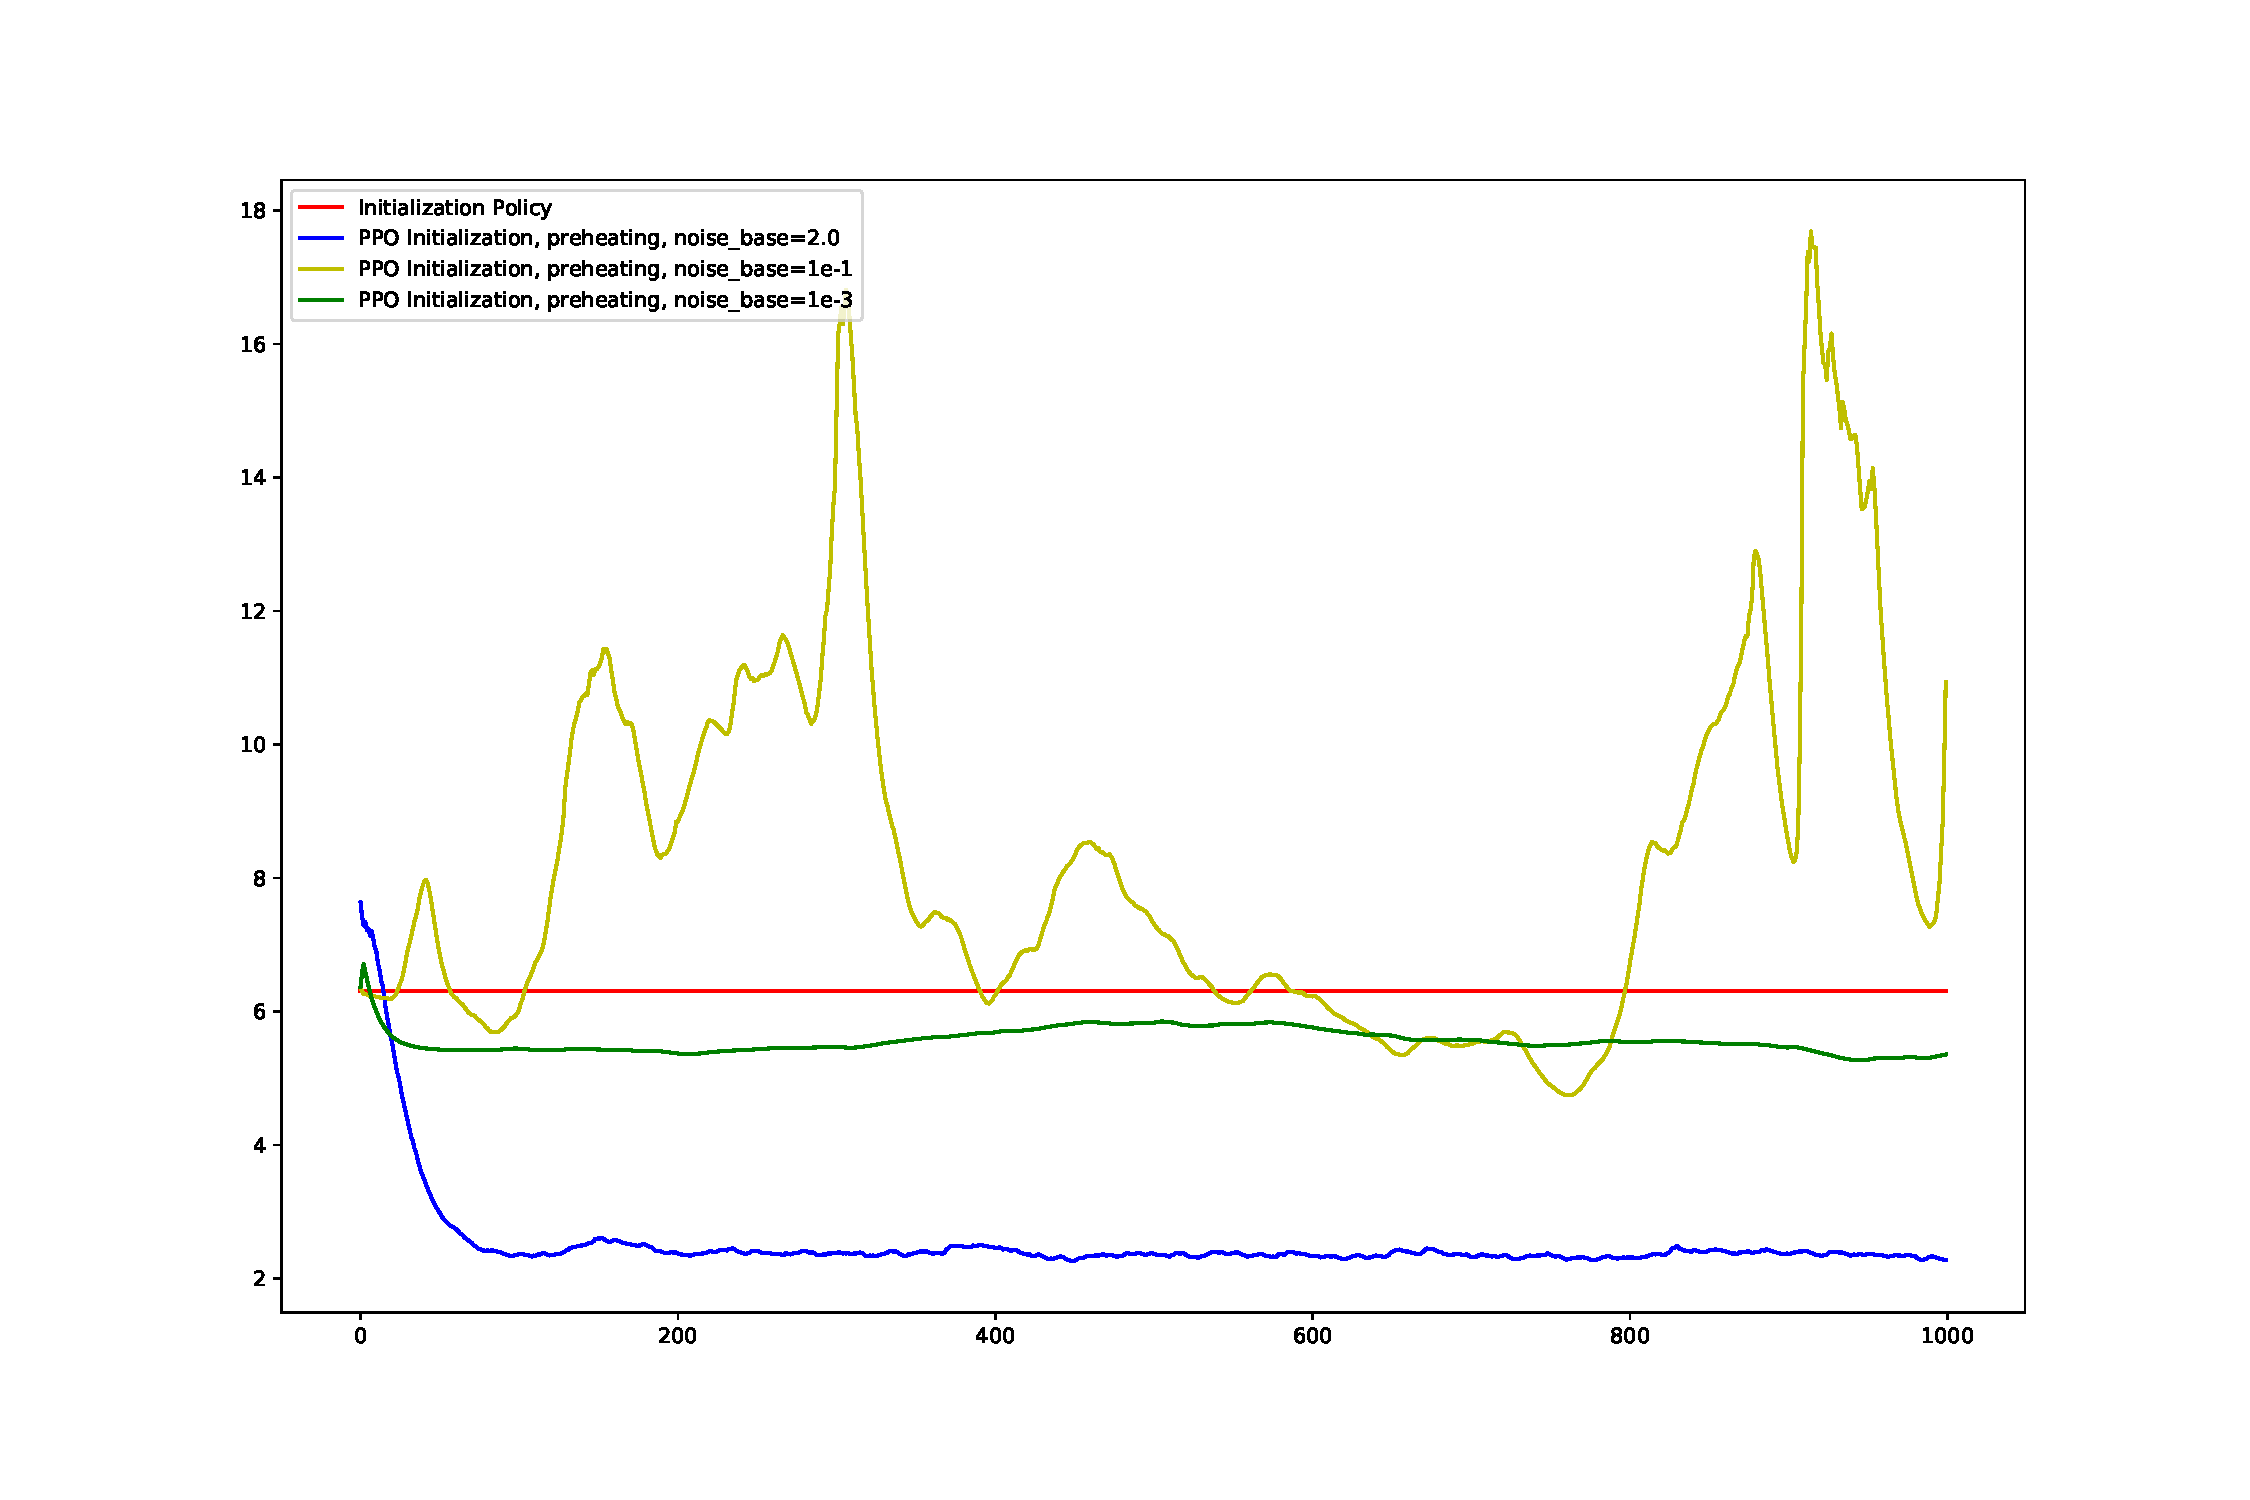
\includegraphics[scale=0.4]{img/ppo_compare4.pdf}
	\caption{Comparison of different noise base for initialized PPO with preheating process on \textit{Reacher} task.}
	\label{fig:ppo3}
\end{figure}

Fig. \ref{fig:ppo3} shows different noise base for initialized PPO. A proper range of noise is needed for effective exploration and learning.


\subsection{Initialized Reinforcement Learning with Supervised Learning Policy -- Residual Policy Learning}
In addition to the policy replacement approach for initialization of RL, residual policy learning \cite{johannink2018residual} is another approach to realize initialization. It s based on good but imperfect controllers for robot manipulation tasks, and to learn a residual policy on top of that initial controller. For robot manipulation in real world, the initial controller could be a pre-trained policy in simulation; and for robot manipulation in simulation, the initial controller could be from the pre-trained supervised learning with expert trajectories as in Section 3.2.

The action in residual policy learning is the sum of the initial policy $\pi_{ini}$ and the residual policy $\pi_{res}$:
\begin{equation}
a=\pi_{ini}(s)+\pi_{res}(s)
\end{equation}
In this way, the residual policy learning is able to preserve the initialized policy performance to the best advantage. Some tricks are applied to guarantee that: 

(1). The weights of the output layer of the actor in RL are initialized to be 0;
 
(2). The same preheating process as in DDPG with initialization: train the critic while fixed the weights of the actor to alleviate the decrease in initial RL training stage caused by a bad critic;

(3). Apply amplification factor for noise scale during the preheating process: for pre-training the critic to have better generalization ability, apply noise multiplied by an amplification factor in the preheating process and reduce it to normal when training the actor.

Note that with above settings, the actor network outputs are actually all 0 during the preheating process, so the action values are fully attributed to the amplified noise and initial policy, which means $\pi_{res}=\epsilon$ and also:
\begin{equation}
a=\pi_{ini}(s)+\alpha * \epsilon, \alpha>1
\end{equation}
where $\epsilon$ denotes the action noise and the $\alpha$ denotes the amplification factor. And the action values stored in the memory (with DDPG algorithm) are $\pi_{res}=\epsilon$ during preheating. This is not a problem as we only train the residual policy $\pi_{res}$ instead of the composite policy $\pi_{ini}+\pi_{res}$, and action values stored in memory are just $\pi_{res}(s)$ instead of the real action value $a$. Correspondingly, the estimated Q-values learned by the critic are also only for the residual policy, which are $Q(s, \pi_{res}(s)))$.

However, there are still several freedoms to be set in residual policy learning, e.g. the scale of the output action from the residual policy can be chosen arbitrarily, which is actually a trade-off between the initialized policy and the learning policy, etc.

\subsubsection{DDPG with Residual Policy Learning}

\subsubsection{Comparison of Residual Learning and Policy Replacement}
We chose the goal position to be easy enough to reach for the agent, in order to shorten the training process and show the overall learning curves, as in Fig. \ref{fig:rpl1}.
\begin{figure}[htbp]
	\centering
	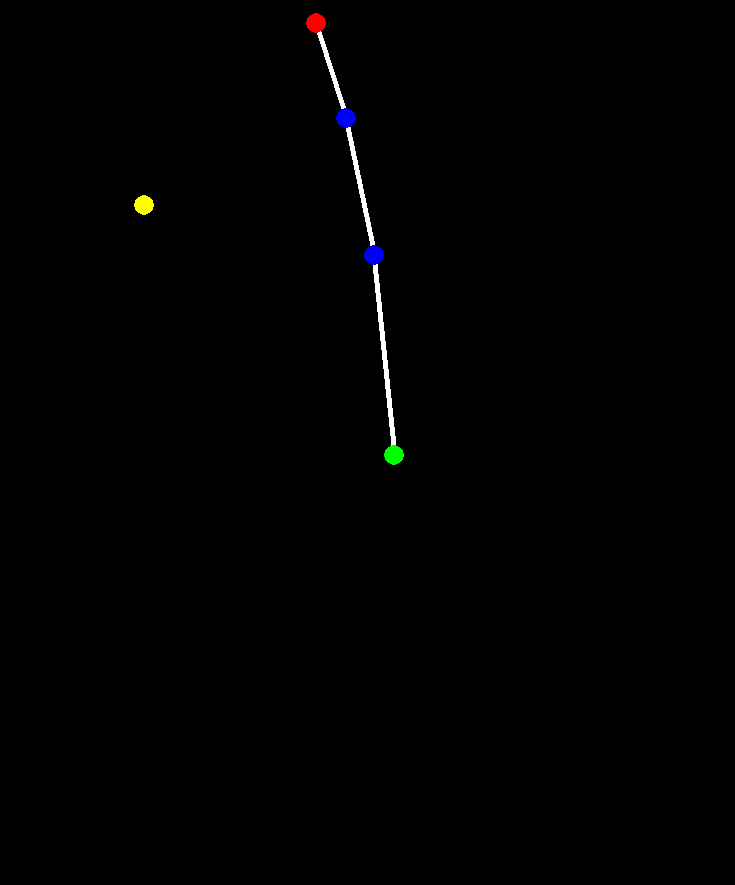
\includegraphics[scale=0.2]{img/goal_position.png}
	\caption{Easy-to-reach goal position used in comparison.}
	\label{fig:rpl1}
\end{figure}

With the same experiment settings: actor learning rate = 1e-4, critic learning rate = 1e-4, steps per episode = 12, same actor and critic network structures, preheating steps = 600 in initialized RL, noise scale = 2.0. The comparisons of non-initialized policy and initialized policy with residual Learning and policy replacement on DDPG for a easy-to-reach goal are shown in Fig. \ref{fig:rpl2}. For some easy-to-reach goals, the policy replacement approach seems to outperform the residual policy learning and non-initialization RL.
\begin{figure}[htbp]
	\centering
	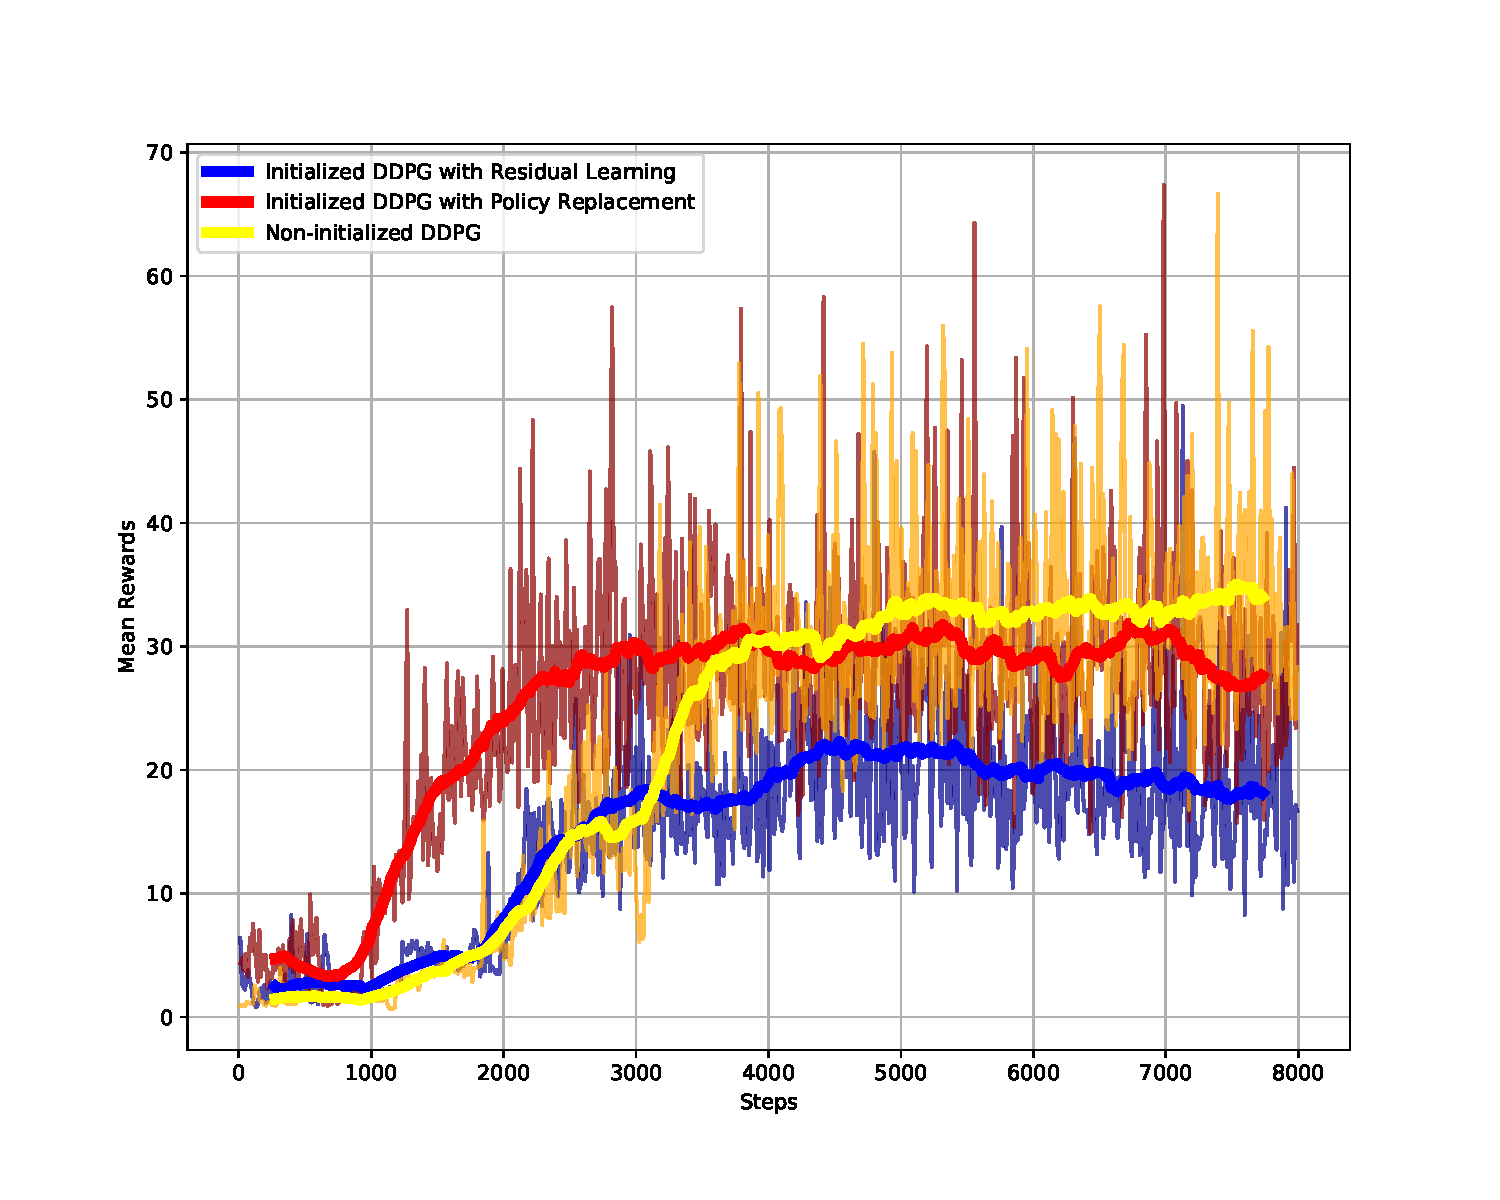
\includegraphics[scale=0.5]{img/res_ddpg3.pdf}
	\caption{Comparison of non-initialized policy and initialized policy with residual learning and policy replacement for DDPG with an easy-to-reach goal position. The bold lines are moving average of episode rewards during learning process. The initialized policy has a preheating process of 600 steps.}
	\label{fig:rpl2}
\end{figure}

Comparison in Fig. \ref{fig:rpl1} shows that, for some goals, initialization with residual learning may not learn as well as policy replacement at the beginning of training, but will eventually learn better policy. This may benefit from the performance guarantee of the initial good policy for residual policy learning, while in policy replacement the learning process may search in a larger trajectories space (testified in observing the experiments). 
\begin{figure}[htbp]
	\centering
	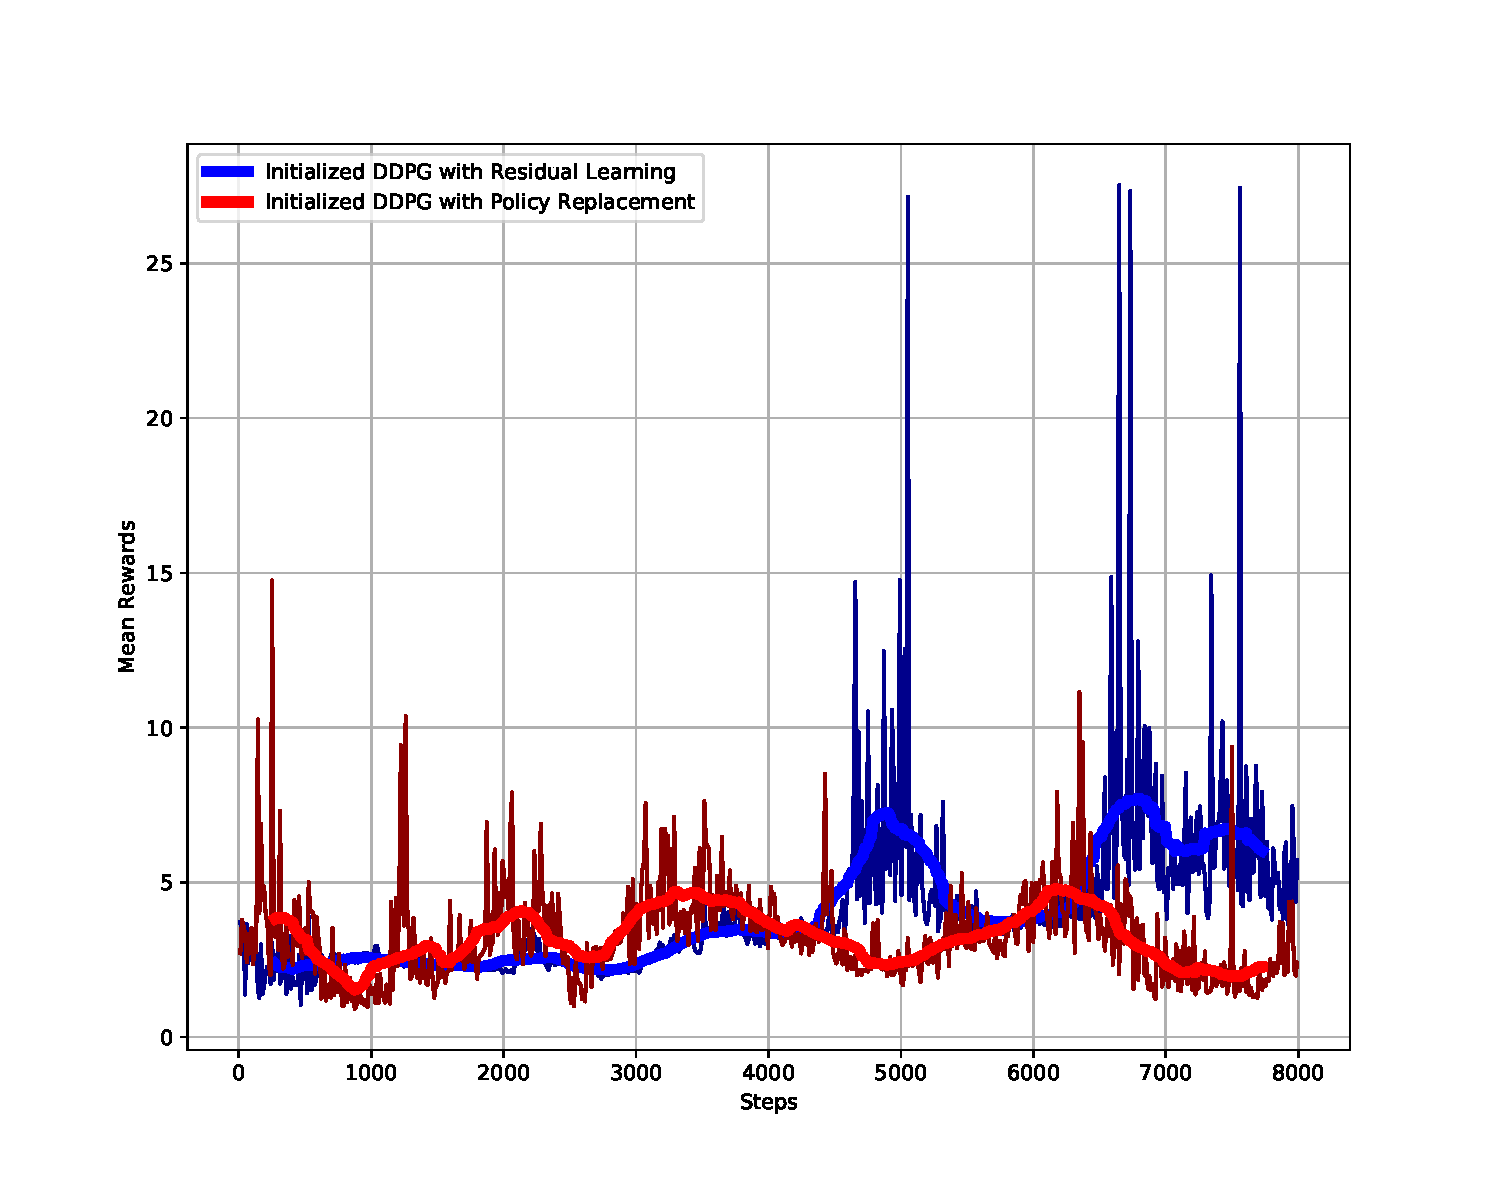
\includegraphics[scale=0.5]{img/res_ddpg2.pdf}
	\caption{Comparison of residual learning and policy replacement for DDPG with another goal position.}
	\label{fig:rpl3}
\end{figure}

With above analysis, we can see that the performances of different approaches to initialize the RL actually have large variance, which are significantly affected by parameters settings and task specifications like goal position, etc. 

\subsubsection{Modelling Analysis of Residual Policy Learning}
Consider that the residual policy learning is actually using policy $\pi_{res}(s)$ to generate the residual action, whose inputs $s$ are exactly the same as the initial policy $\pi_{ini}(s)$, the modelling of residual policy is actually may be more complicated than a general policy in RL, although the value range of outputs for residual policy may be smaller (a smaller searching space for delicate actions). In order to have a more accurate composite action, the residual policy not only needs to model the environment but also the initial policy. The modelling relationship can be interpreted as follows. 

We denote the modelling of a general policy in RL as $\mathcal{M}_g$, the modellings of the initial policy and the residual policy are $\mathcal{M}_i, \mathcal{M}_r$, respectively. A modelling means a mechanism that the policy learned from interactions with its environment to represent the its environment and based on which the policy determines actions. The relationship of above modellings is:
\begin{equation}
	\mathcal{M}_g = \mathcal{M}_i \oplus \mathcal{M}_r
 \end{equation}
 which means the $\mathcal{M}_i, \mathcal{M}_r$ are actually dual modellings with respect to a $\mathcal{M}_g$. As we only train the residual policy in the learning process of residual RL, we have the modelling to construct in this training process the $\mathcal{M}_r$:
 \begin{equation}
 \mathcal{M}_r = \mathcal{M}_g \ominus \mathcal{M}_i
 \end{equation}
 where the $\oplus, \ominus$ denotes a positive or negative modelling composite relationship. And the composite relationship does not determine the complexity of the composite modelling to be more or less than original constituent modellings, which means the modelling of $\mathcal{M}_r$ may not be less complicated than the general policy $\mathcal{M}_g$, and sometimes even more complicated than $\mathcal{M}_g$. This means the learning of a residual does not have to be easier than directly learning the general policy.
 
 The $\textit{Reacher}$ task is made more complicated for testing effects of demonstrations, in which there are two penalty areas. Fig. shown comparisons of DDPG from demonstrations with general DDPG, both without prioritized experience replay.

\subsection{Meta-learning as Initialization for Reinforcement Learning}

\subsubsection{MAML and Reptile}

\subsubsection{Reptile + PPO}

\subsection{Off-Policy Reinforcement Learning with Demonstrations}
We show different initialization strategies for efficient RL as above, and leveraging demonstrations for deep RL is an alternative approach to learn efficiently. Both initialization approach and leveraging demonstrations approach are taking advantages of the expert trajectories, however, they treat them differently. Instead of pre-training a policy to initialize the RL policy, the approach of leveraging demonstrations directly feeds those expert trajectories into memory of off-policy RL (e.g. DDPG) to make the policy trained with both demonstrations and explorations.

We apply a more complicated environment for this experiment as shown in Fig. \ref{fig:ddpgfd0}, with two penalty areas. The optimal trajectories for the agent is to go through the middle of two penalty areas. And we generate good demonstrations by manually setting an intermediate goal position at the middle of two penalty areas.

Experiment results of applying DDPG from demonstrations with different feeding approaches and vanilla DDPG are shown in Fig. \ref{fig:ddpgfd1}.  The prioritized experience replay is not used in this experiment. The feeded demonstration dataset contains totally 50 episodes (20 steps each episode) of trajectories, and each feeding operation is to feed the whole demonstrations dataset. It seems the more demonstrations feeded into the memory, the worst learning performance it is.
\begin{figure}[htbp]
	\centering
	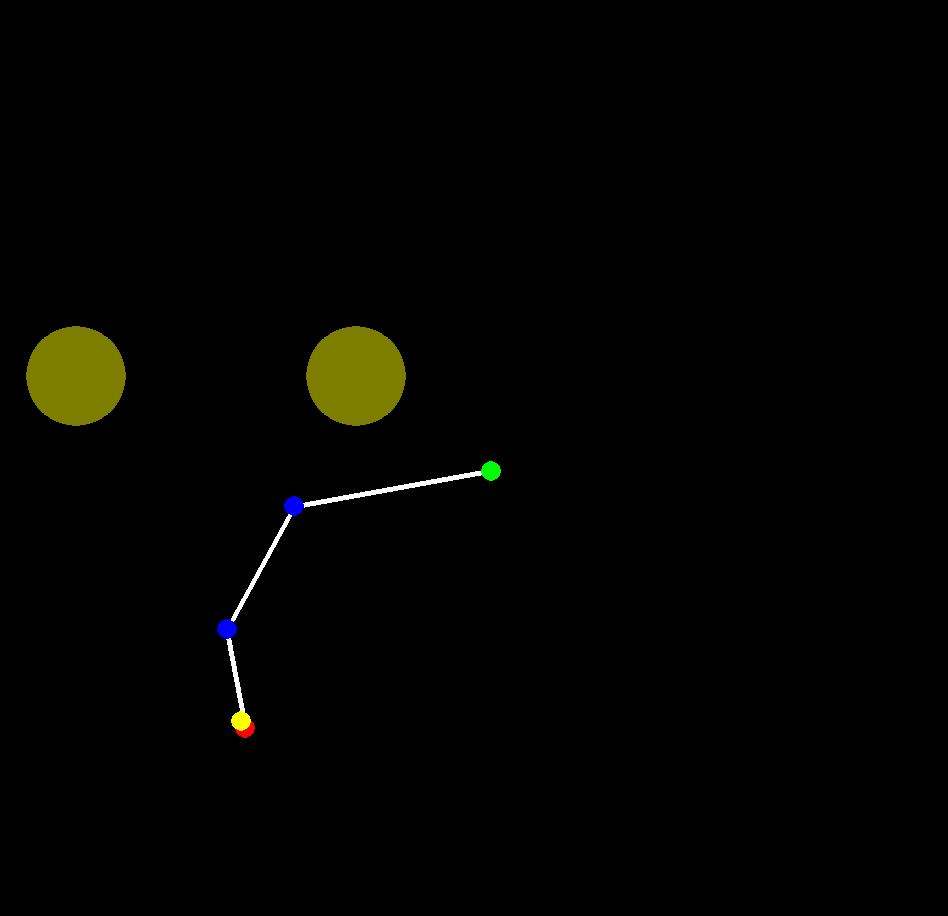
\includegraphics[scale=0.3]{img/ddpgfd_env.png}
	\caption{$\textit{Reacher}$ environment with two penalty areas.}
	\label{fig:ddpgfd0}
\end{figure}

\begin{figure}[htbp]
	\centering
	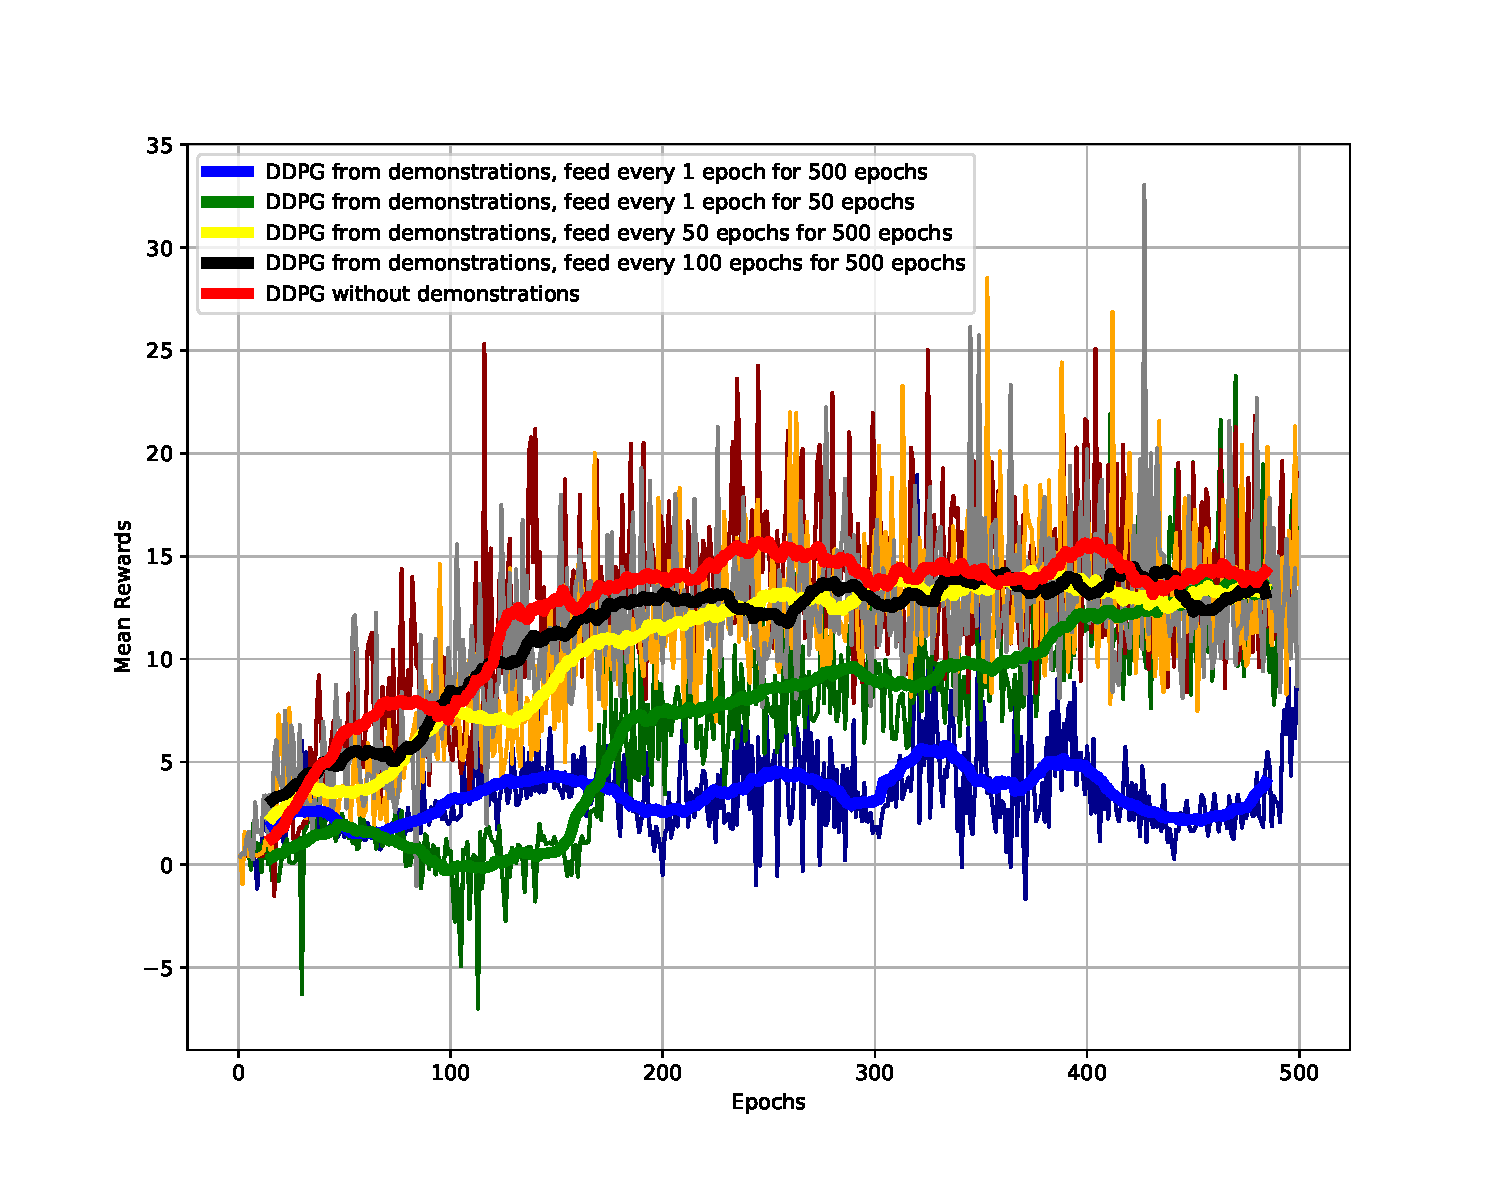
\includegraphics[scale=0.5]{img/ddpgfd1.pdf}
	\caption{Comparison of DDPG from demonstrations with different feeding approaches (without prioritized experience replay) and vanilla DDPG. The blue line is feeding demonstrations for every epoch for the whole training process (500 epochs); the green line is feeding demonstrations for every epoch for the first 50 epochs; the yellow line is feeding demonstrations for every 50 epochs for the whole training process; the black line is feeding demonstrations for every 100 epochs for the whole training process; the red line is vanilla DDPG without using demonstrations. }
	\label{fig:ddpgfd1}
\end{figure}



\medskip
 
\bibliographystyle{unsrt}
\bibliography{ref}

\end{document}
